\documentclass[a4paper,12pt]{atuaref}
%\documentclass[a4paper,12pt,russian]{atuaref}
\RequirePackage[utf8]{inputenc}
\usepackage[verbose,tmargin=25mm,bmargin=25mm,lmargin=30mm,rmargin=20mm,headsep=10pt]{geometry}
% example: W=125mm, H=180mm
\newlength\TW
\setlength{\TW}{0.01\textwidth} % after geometry!
\usepackage{amssymb}
\usepackage{amsmath}
\usepackage{amsthm}
\usepackage{bropd} % od, pd
\usepackage{tabularx}
\usepackage{fouriernc}
\usepackage{paratype}

\usepackage{graphicx}
\usepackage{tikz}
%\usepackage[english,russian,ukraineb]{babel}
\usepackage[english,ukraineb,russian]{babel}

\usepackage[backend=biber,language=russian,sorting=none,maxnames=10,bibstyle=gost-numeric]{biblatex}

\usepackage{blox}
\usepackage[europeanresistors,americaninductors,siunitx,fulldiodes]{circuitikz}

\usetikzlibrary{calc}
\usetikzlibrary{arrows}
\usetikzlibrary{patterns}
%\usepgflibrary{shapes.geometric}
\usetikzlibrary{external}


\definecolor{haircolor}{rgb}{0.7,0.7,1.0}
\newcommand{\TikzAddPadding}{\path (current bounding box.north east) ++(+0.1,+0.1); \path (current bounding box.south west) ++(-0.1,-0.1);}

\tikzset{
  >=stealth,
  %semiRed/.style={fill=red,opacity=0.3,draw=black,thin},
  hair/.style={draw,color=haircolor,line width=0.1pt},
  medline/.style={draw=black,line width=0.6pt},
  medlinep/.style={draw=black,line width=0.6pt,->},
  semiboldline/.style={draw=black,line width=1.2pt},
  semiboldlinep/.style={draw=black,line width=1.2pt,->},
  infoline/.style={draw=gray,line width=1.4pt},
  boldline/.style={draw=black,line width=2.0pt},
  boldlinep/.style={draw=black,line width=2.0pt,->},
  wire/.style={draw=black,line width=1.0pt},
  elelem/.style={draw=black,line width=1.5pt},
  subelem/.style={draw=black,dashed,line width=0.6pt}
}



\newcommand{\booknameUa}{Ансамблеві пошукові моделі і методи параметричної ідентифікації систем з хаотичною поведінкою}
\newcommand{\booknameRu}{Ансамблевые поисковые модели и методы параметрической идентификации систем с хаотическим поведением}
\newcommand{\booknameEn}{Ensemble search models and methods for parametric identification of systems with chaotic behavior}
\newcommand{\bookname}{\booknameRu}

\newcommand{\bookyear}{2018}
\newcommand{\dissauthorUa}{Гуда~А.І.}
\newcommand{\dissauthorRu}{Гуда~А.И.}
\newcommand{\dissauthorEn}{Guda~A.I.}
\newcommand{\dissauthorFullRu}{Гуда Антон Игоревич}
\newcommand{\dissauthorFullUa}{Гуда Антон Ігорович}
\newcommand{\dissauthorMain}{\dissauthorRu}
\newcommand{\dissauthorAref}{\dissauthorUa}
\newcommand{\dissauthorFullMain}{\dissauthorFullRu}
\newcommand{\dissauthorFullAref}{\dissauthorFullUa}

\newcommand{\dissSpecUa}{математичне    моделювання  та обчислювальні методи}
\newcommand{\dissSpecRu}{математическое моделирование и вычислительные методы}
\newcommand{\dissSpecEn}{Mathematical Modelling and Computational Methods}
\newcommand{\dissSpecMain}{\dissSpecRu}
\newcommand{\dissSpecAref}{\dissSpecUa}
\newcommand{\dissSpecId}{01.05.02}
\newcommand{\dissScopeRu}{технических наук}
\newcommand{\dissScopeUa}{техничних наук}
\newcommand{\dissScopeMain}{\dissScopeRu}
\newcommand{\dissScopeAref}{\dissScopeUa}
\newcommand{\UDC}{004: 681.5.015}
\newcommand{\dissRada}{Д.~08.084.01}
\newcommand{\dissSekrRadi}{Селівьорстова~Т.В.}
\newcommand{\institutionRu}{Национальная металлургическая академия Украины}
\newcommand{\institutionUa}{Національна  металургійна     академія України}
\newcommand{\institutionEn}{National Metallurgical academy of Ukraine}
\newcommand{\institutionMain}{\institutionRu}
\newcommand{\institutionAref}{\institutionUa}
\newcommand{\belongRu}{Министерство образования и науки Украины}
\newcommand{\belongUa}{Міністерство освіти і науки      України}
\newcommand{\belongEn}{Ministry of Education and Science of Ukraine}
\newcommand{\belongMain}{\belongRu}
\newcommand{\belongAref}{\belongUa}
\newcommand{\cityRu}{Днепр}
\newcommand{\cityUa}{Дніпро}
\newcommand{\cityEn}{Dnipro}
\newcommand{\cityMain}{\cityRu}
\newcommand{\cityAref}{\cityUa}
\newcommand{\superRu}{Михалёв Александр Ильич}
\newcommand{\superUa}{Михальов Олександр Ілліч}
\newcommand{\superMain}{\superRu}
\newcommand{\superAref}{\superUa}


\renewcommand{\Rada}{\dissRada}
\renewcommand{\SekrRadi}{\dissSekrRadi}

\author{\dissauthorFullAref}

\title{\booknameUa}
\date{\bookyear}

\addbibresource{atuworks.bib}

\DeclareMathOperator*{\sign}{sign}

\newcommand{\TermDef}[1]{\textit{\textbf{#1}}}
\newcommand{\TermUse}[1]{\textit{#1}}
\newcommand{\ProgName}[1]{\textsl{#1}}
\newcommand{\xsect}[1]{\medskip\begin{center}\textbf{#1}\end{center}\medskip\penalty10000}
%\newcommand{\xxsect}[1]{\smallskip\begin{center}\textbf{#1}\end{center}\smallskip\penalty10000}
\newcommand{\xxsect}[1]{\smallskip\textbf{#1}\smallskip\penalty10000}


\begin{document}

\sloppy

\thispagestyle{empty}
\begin{center}

\textbf{\belongAref}

\vspace{1ex}

\textbf{\institutionAref}

\vspace{3ex}

\textbf{\dissauthorFullAref}

\end{center}

\vspace{3ex}

\begin{flushright}
УДК \UDC
\end{flushright}

\vfill

\begin{center}
\textbf{\Large
\booknameUa
}

\vfill

\dissSpecId --- \dissSpecAref

\vfill

\textbf{Автореферат} \\
\textbf{  дисертації на здобуття наукового ступеня }\\
\textbf{доктора \dissScopeAref }


\vfill

\cityAref --- \bookyear

\end{center}

\clearpage

\thispagestyle{empty}

\noindent
Дисертацією є рукопис

\vspace{3ex plus 2ex}

\noindent
Робота виконана в Національній металургійній академії України
Міністерства освіти і науки України.


\vspace{4ex plus 4ex}

\noindent
\begin{tabular}{lp{0.64\textwidth}}
\textbf{Науковий консультант:}
&
доктор технічних наук, професор,\newline
\textbf{Михальов Олександр Ілліч,}\newline
Національна металургійна академія України,
завідувач кафедри інформаційних технологій і систем.
\\
{~} & {~}
\\
\textbf{Офіційні опоненти:}
{~}
&
доктор фіз.-мат. наук, професор,\newline
\textbf{XXX}
професор .
\\
{~} & {~}
\\
&
доктор технічних наук, професор,\newline
\textbf{XXX},
  ---
\\
{~} & {~}
\\
{~}
&
доктор технічних наук, професор,\newline
% \textbf{Жолткевич Григорій Миколайович},
%   декан механіко-математичного факультету,
%   завідувач кафедри теоретичної та прикладної інформатики
%   Харківського національного університету ім.~В.Н.~Каразіна;
\end{tabular}

\vspace{5ex plus 4ex}


\vfill

Захист відбудеться
<<\_\_\_\_>>
~\_\_\_\_\_\_\_\_\_\_\_
\bookyear~р. о \_\_\_\_ годині
на засіданні спеціалізованої вченої ради Д 08.084.01 у Національній
металургійній академії України за адресою: 49600, м.~\cityUa,
пр.~Гагаріна,~4.


\vspace{4ex plus 3ex}
З дисертацією можна ознайомитись у бібліотеці Національної металургійної
академії України за адресою: 49600, м.~\cityUa, пр.~Гагаріна,~4.

\vspace{4ex plus 3ex}
Автореферат розісланий 
<<\_\_\_\_>>
~\_\_\_\_\_\_\_\_\_\_\_
\bookyear~р.

\vspace{4ex plus 3ex}

\begin{tabular}{p{0.44\textwidth}p{0.2\textwidth}p{0.35\textwidth}}
Вчений секретар спеціалізованої вченої ради 
&
{~}
&
\SekrRadi
\end{tabular}

\vspace{2ex}

\clearpage


\setcounter{page}{1}

\xsect{ЗАГАЛЬНА ХАРАКТЕРИСТИКА РОБОТИ}

\textbf{Актуальність роботи.}
Нелінійні динамічні системи, широко представлені в сучасних технологічних і
природних процесах, незважаючи на детермінізм їх визначення, можуть проявляти
хаотичні властивості в своїй динаміці. При цьому як завгодно малі збурення у вхідних
впливах і параметрах самої системи призводять до значних, але кінцевим збуренням
вихідного сигналу. Це призводить до певних труднощів при конструюванні,
управлінні і прогнозі поведінки таких систем.

При математичному та комп'ютерному моделюванні систем динамічного хаосу
виникають специфічні для даних систем проблеми. Перш за все --- потрібно
забезпечити наявність працездатного критерію адекватності моделі. Для задач
ідентифікації наявність такого критерію є принциповим. Найбільш часто
використовувані при моделюванні поведінки динамічних систем критерії, засновані
на звичних заходи в просторі вихідних сигналів, виявляються непрацездатними. З
іншого боку, спеціальні характеристики оцінювання хаотичних властивостей динамічних
систем, такі як фрактальна розмірність, показник Ляпунова, перетин Пуанкаре,
недостатньо інформативні для задачі ідентифікації через обмежений діапазон
змін, великою похибкою при їх вимірі для реальних систем і суттєвою
обчислювальною складністю.

У якості прототипу для синтезу нових методів ідентифікації доцільно обрати ряд
методів ідентифікації, які було розроблено та досліджено у роботах
П.~Ейкхоффа, Л.А.~Растрігіна, Л.Н.~Фіцнера, Е.Є.~Гачинського,
А.І.~Дроздова, О.І.~Михальова, зокрема пошукові та адаптивно-пошукові
методи.
Також вважається доцільним використання як основи
наступного класу двомодельних адаптивно-пошукових методів,
які було розроблено та досліджено у попередньої роботі.
Проте, результати моделювання процесів ідентифікації цими методами
технічних об'єктів, які проявляють складну та хаотичну динаміку, показали
їх повну або обмежену непридатність.


Тому проблема ідентифікації динамічних систем, які проявляють хаотичну
динаміку, або близьку до хаотичної, є
\textit{актуальною}.

\smallskip
\textbf{Зв'язок роботи з науковими програмами, планами, темами.}
Дисертаційна робота виконувалась у рамках науково-дослідних робіт
Національної металургійної академії України за держбюджетною
тематикою:

\begin{itemize}


\item
  ``Вдосконалення технології утилізації в металургійній промисловості
  матеріальних і енергетичних відходів'', №~держ. реєст. 0113U003266;

  \item
  ``Дослідження та імітаційне моделювання процесів нелінійної динаміки
  формування фрактальних структур функціональних   покриттів'',
  № держ. реєст. 0110U003240;

  \item
  ``Наукове обґрунтування та розробка ефективних тепло-масообмінних
  процесів в інноваційних металургійних технологіях'', №~держ. реєст 0115 U003176.

\end{itemize}

Результати було впроваджено у рамках науково-практичного дослідження
``Оцінка    можливості заміни випробувань КА на стійкість до акустичного навантаження
випробуваннями широкосмугової вібрації'', згідно договору №~V-105-16-3 від 07.09.2016.

\textbf{Мета і задачі дослідження.}
Головною метою дослідження є створення нових методів ідентифікації з
використанням адаптивно-пошукових принципів настроювання параметрів, які
були б придатні для створення моделей систем, які проявляють хаотичну
та/або схожу на хаотичну динаміку. В свою чергу, окремо ставиться задача
розв'язання наукової проблеми створення адекватних моделей процесів
ідентифікації хаотичних систем з використанням запропонованих нових
методів, аналізу та дослідження їх характеристик в умовах невизначеності.

Для досягнення даної мети були поставлені наступні задачі:

\begin{itemize}

  \item
  розробити нові критерії ідентифікації, які, на відміну від тих, що
  існують, при моделюванні були б придатні для аналізу стану та динаміки
  хаотичних систем, що створить обґрунтування працездатності систем
  ідентифікації;

  \item
  розвинути існуючи та розробити нові методи пошуку, які б не мали
  обмежень тих, що існують, та у повної мірі використовували можливості
  паралельних обчислювань та переваг використання ансамблю
  синергированних моделей;

  \item
  розвинути існуючи та розробити нові методи адаптації параметрів
  системи ідентифікації, здатні пристосуватися до зміни режимів роботи
  системи;

  \item
  розробити програмне забезпечення, придатне для моделювання як систем
  хаотичної динаміки, так і систем ідентифікації;

  \item
  провести комп'ютерне моделювання процесів ідентифікації систем
  хаотичної динаміки та дослідити їх працездатність, можливості та
  характеристики.

\end{itemize}


\textbf{Об'єктом дослідження є}
технічні системи, які в процесі їх функціювання можуть
входити в хаотичні режими.

\smallskip
\textbf{Предметом дослідження є}
математичні моделі процесів та методи
адаптивно-пошукової ідентифікації технічних систем з хаотичною динамікою.

\smallskip
\textbf{Методи дослідження.}
Для вирішення поставлених задач використовувався математичний апарат
теорії управління та ідентифікації нелінійних систем, динамічного хаосу,
обчислювальних методів, нечіткої логіки, теорії інформації тощо.

\smallskip
\textbf{Наукова новизна одержаних результатів:}
Основний науковий результат полягає в розв'язанні науково-практичної проблеми
синтезу методів ідентифікації
технічних систем хаотичної динаміки, створенні відповідних математичних
моделей та дослідженні результатів моделювання процесів
адаптивно-пошукової ідентифікації.

Основні наукові результати, що отримані в дисертаційної роботі, полягають
в наступному:

\noindent
вперше:

\begin{itemize}

  \item
  створено критерії ідентифікації нелінійних динамічних систем,
  які, на відміну від тих, що існують, дозволяють оцінити їх стан та
  хаотичну динаміку, та дають підстави для створення ефективних алгоритмів
  настроювання параметрів моделей систем ідентифікації;

  \item
  створено методи адаптивно-пошукової ідентифікації на підставі
  адаптивно-пошукової парадигми з використанням ансамблю пошукових агентів,
  які взаємодіють проміж собою, які на відміну від методів, що використовують
  одну модель або пару моделей, значно підвищують швидкість пошуку та
  здатні за мінімальний час перестрілюватися при різкої зміні параметра, а на
  відміну від ройових алгоритмів, нові методи потребують значно меншої
  кількості моделей та забезпечують певні гарантії пошуку;

  \item
  створено нову класифікацію систем ідентифікації динамічних систем,
  яка як вбирає у себе методи, що існують, так і дозволяє
  створювати нові методи ідентифікації за рахунок
  комбінування їх складових частин;

  \item
   визначено, що системи з сухим тертям з точки зору задачі ідентифікації
   при певних  умовах функціонування
   мають властивості, що поєднують їх з системами хаотичної динаміки, тобто з
   системами хаотичної динаміки їх поєднує суттєва залежність від початкових
   умов та вид атрактору, що також потребує використання нових методів ідентифікації;

  \item
   запропоновано модель системи хаотичної динаміки системи зв'язаних релаксаційних генераторів,
   яка відрізняєшся від існуючих відсутністю індуктивних компонентів,
   працездатністю при малих напругах та можливістю
   керування частотним діапазоном у широкому діапазоні,
   що сприяє процесу аналізу хаотичної динаміки
   фізичного об'єкту, перевірки адекватності математичної моделі
   та властивостей системи ідентифікації стосовно цієї системи.
\end{itemize}

\noindent
Набуло подальший розвиток:
\begin{itemize}

  \item
  методи оцінювання якості ідентифікації,
  які на відміну від тих, що існують,
  враховують використання множини агентів;

  \item
  підходи до адаптації параметрів систем
  адаптивно-пошукової ідентифікації, які придатні використовувати поточну
  інформацію від ансамблю сінергированих моделей, та корегувати глобальні
  параметри пошуку;

  \item
    модель генератора Копітца, яка враховує
    більшу кількість нелінійних ефектів,
    що забезпечує більш адекватні результати процесу
    ідентифікації її параметрів новими методами;

\end{itemize}


\smallskip
\textbf{Практичне значення одержаних результатів.}
Розроблені методи ідентифікації було використано
при проектуванні, створенні, налаштовуванні параметрів
стенду дослідження вібраційного та акустичного впливу.
Аналіз результатів даних з цього стенду
дав можливість указати потрібні нелінійні властивості системи,
та діапазон параметрів, які у сукупності
забезпечують широкосмуговий спектр коливань.

Створене програмне середовище для моделювання нелінійних динамічних систем
використається при проведенні практичних робіт по дисциплінам
``Моделювання систем'',
``Сучасні системи управління'' на кафедри інформаційних технологій
і систем Національної металургійної академії України.


\smallskip
\textbf{Особистий внесок здобувача.}

Усі основні положення і результати
дисертаційної роботи, які виносяться на захист, отримано здобувачем особисто та
опубліковано в роботах [1--49]. У наукових працях, опублікованих у співавторстві,
здобувачу належать наступні результати. У роботі [1] \ldots



\smallskip
\textbf{Апробація результатів.}
Основні положення дисертаційної роботи доповідались на наукових
семінарах кафедри ІТС,
регіональному науковому семінарі Придніпровського Наукового Центру НАН України
''Сучасні проблеми управління та моделювання складних систем'',
науково-практичних коференціях:
``Інформатика та системні науки'' (ІСН-2011) Полтава--2011,
``Интеллектуальные системы принятия решений и проблемы вычислительного интеллекта'' (ISDMCI) Херсон--2011,
``Информационные технологии в управлении сложными системами'' Днепропетровск--2011,
``Автоматизация: проблемы, идеи, решения'' Севастополь-2011,
``Интеллектуальные системы принятия решений и проблемы вычислительного интеллекта'' (ISDMCI) Херсон--2012,
``Автоматизация: проблемы, идеи, решения'' Севастополь-2012,
``Интеллектуальные системы принятия решений и проблемы вычислительного интеллекта'' (ISDMCI) Херсон--2013,
``Автоматизация: проблемы, идеи, решения'' Севастополь-2013,
``Интеллектуальные системы принятия решений и проблемы вычислительного интеллекта'' (ISDMCI) Херсон--2014,
``Интеллектуальные системы принятия решений и проблемы вычислительного интеллекта'' (ISDMCI) Херсон--2015,
``Computer Sciences and Information Technologies'' (CSIT) Lviv--2015 (Scopus),
``Интеллектуальные системы принятия решений и проблемы вычислительного интеллекта'' (ISDMCI) Херсон--2016,
``Data Stream Mining and Processing'' DSMP Lviv-2016 (Scopus,Web of Science).

\smallskip
\textbf{Публікації.}
По темі дисертації опубліковано
49 друкована праця,
з них
24 входять до до міжнародних наукометрічних баз,
13 статей опубліковано у матеріалах конференцій.

\smallskip
\textbf{Структура і обсяг роботи.}
Дисертація складається з вступу, 6 розділів, що викладені на
XXX сторінках, висновків, списку літературних джерел з
XX найменувань,
1 додатка.
Робота проілюстрована XXX рисунками.


\xsect{ОСНОВНИЙ ЗМІСТ РОБОТИ}

У \textbf{вступі} обґрунтовано актуальність теми,
сформульованл цілі і задачі дослідження,
відзначені наукова новизна і практична цінність роботи, відображені
одержані результати, що виносяться на захист.

У \textbf{першому розділі}
проведено аналітичний огляд проблем
влстивостей систем хаотчної динаміки
з точки зору задачі ідентифікації.

Проведено аналіз публікації, розглянуто методb ідентификації, що існують.
Розглянуто причини, які на дозволяють використовувоти ці методи для
ідентифицації систем динаміного хаосу, а також складних нехаотичних систем, які
з точки зору ідентификації мають з ними певні загальні риси.  Проведено аналіз
методів оцінювання якості ідентифікації, у тому числі інформаціїних.




\textbf{Другий розділ}
присвячено розробці та досліженню як елементів систем ідентификації,
що здатні працювати з системам хаотичної динаміки, так і системи іднтифікаціі у цілому.

По-перше, досліджуються крітерії ідентификації,
які мають сенс при роботі с системами
хаотичної динаміки.
Особливість динаміки хаотичних систем не дозволяє визначити мету ідентифікації
як задачу мінімізації будь-якої міри
$ \mu (x_o (t), x_i (t)) $ в просторі
вихідних сигналів~\cite{atu_asau11, atu_asau12, atu_asau14}.

Отже, для синтезу системи ідентифікації необхідно існування заданого скалярного
критерію $q(x(t)) $, близькість величин яких для об'єкта і моделі (в сенсі
будь-якої міри) і дозволяє говорити про досягнення мети ідентифікації.

Для створення можливості використання критерію для цілей ідентифікації
динамічних системи, сам критерій повинен якимось чином відображати глобальні
властивості системи, а не її стану в конкретний момент часу, тобто не
змінюватися (принаймні істотно), якщо властивості системи, що пред'являються в
математички моделі параметрами, не змінюються. У таких випадках має сенс
використовувати термін ``інтегральні критерії''.
Для досить простих систем вид критерію, придатного для задачі ідентифікації,
можна вивести, визначивши будь-яким чином виходячи зі структури математичної
моделі. У деяких випадках випадках вид критерію можна підібрати емпірично, на
підставі досвіду в синтезі систем ідентифікації для подібних систем. Проте,
найбільш обгрунтованим є підхід, заснований на використанні будь-яких фізичних
інваріантів.
Найбільш загальним, і, отже, найбільш вживаним є закон збереження енергії.

Розглянемо основні способи подання енергії:

Кінетична енергія тіла масою $m$, яке рухається зі швидкістю $v$:
%
\begin{equation}
  E_k = \frac{mv^2}{2} = \frac{m}{2} \left( \od{x}{t} \right)^2.
  \label{atu:eq:Ek_v}
\end{equation}
%

Потенційна енергія в однорідному полі (нульовий рівень вибирається довільно):
%
\begin{equation}
  E_p = m g x .
  \label{atu:eq:Ep_g}
\end{equation}

Потенційна енергія в пружному наближенні:
%
\begin{equation}
  E_p = k \frac{x^2}{2} .
  \label{atu:eq:Ep_spring}
\end{equation}

Кінетична енергія тіла, що обертається:
%
\begin{equation}
  E_k = J \frac{\omega^2}{2} = \frac{J}{2} \left( \od{\varphi}{t} \right)^2 .
  \label{atu:eq:Ek_spin}
\end{equation}

Внутрішня теплова енергія:
%
\begin{equation}
  E_t = \frac{im}{2M} RT.
  \label{atu:eq:Et}
\end{equation}

Електрична енергія, накопичена в конденсаторі:
%
\begin{equation}
  E_c = \frac{C U^2}{2}.
  \label{atu:eq:Ec}
\end{equation}

Енергія магнітного поля, накопичена в котушці індуктивності:
%
\begin{equation}
  E_l = \frac{L I^2}{2} = \frac{L}{2} \left( \od{Q}{t}\right)^2 .
  \label{atu:eq:El}
\end{equation}

Енергія, яка перетворюється у тепло омічним опором:
%
\begin{equation}
  E_r = U I = I^2 R = \frac{U^2}{R} = U \od{Q}{t} .
  \label{atu:eq:Er}
\end{equation}

Узагальнюючи вищевикладене, можна зробити висновок, що незважаючи на
різноманітність фізичних процесів, кількість способів подання енергії
(розглядаємо зосереджені параметри) досить обмежена. Основні види залежностей:

\begin{itemize}

  \item
  Квадратична залежність від координати:
    $E \sim x^2$.

  \item
  Лінійна залежність від координати:
    $E \sim x$.

  \item
  Квадратична залежність від похідної координаты по часу:
    $E \sim \left( \od{x}{t}\right)^2$.

  \item
  Лінійна залежність від добутка координат:
    $E \sim x \cdot y$.

  \item
    Лінійна залежність від добутка ожнієї координати на похідну іншої:
     $E \sim x \cdot \od{y}{t}$.

  \item
  Максимум величини на заданому інтервалі часу.

\end{itemize}

Поняття інтегрального критерію, що застосовується до реальних завдань, має на
увазі не тільки власне взяття або оцінку інтеграла та обраному часовому
інтервалі, а й нормування на величину цього інтеграла. Це дає можливість
застосовуваним критеріям не мати явної мультипликативной залежності від часу, і
описувати власне властивості об'єкта. Таким чином, інтегральний критерій можна
уявити як різновид усереднення для вираження, що формує цей критерій.

Найбільш очевидний спосіб обмеженого за часом усереднення --- ковзне середнє. У
застосовуваних термінах, якщо базове вираз для формування критерію позначити як
$ x(t)$, то цей спосіб усереднення має вигляд:
%
\begin{equation}
  q_{x,a}(t) =
  \frac{1}{\tau_q}
  \int\limits_{t-\tau_q}^{t} x(t) \, dt.
  \label{atu:eq:moving_avarage}
\end{equation}

Менш витратним (з точки зору обсягу обчислень) є метод експоненціального
згладжування, динаміку якого стосовно сигналу $x(t) $ можна описати
рівнянням:
%
\begin{equation}
\od{q_{x,l}}{t}
=
\frac{1}{\tau_q} \left( x(t) - q_{x,l}(t) \right)
\label{atu:eq:qlin}
\end{equation}

На перший погляд, при заданому критерії ідентифікації, завдання ідентифікації
зводиться до класичної задачі розв'язання нелінійного рівняння: треба знайти
такі значення параметрів $ p $, при яких критерій моделі (або будь-якої з
моделей) $ q_m $ приймає значення, найбільш близьке до значення критерію
об'єкта $ q_o $:
\[
  \mu( q_o, q_m(p) ) \to \min.
\]

Насправді, існують певні аспекти, які роблять таке зведення практично
неможливим. Перш за все, в завданню в обох вихідних задачах передбачається, що
спостережувана система статична: значення критерію не залежить від часу, і
провівши вимір в точці один раз, можна до нього не повертатися. Навпаки,
ідентифікація динамічної системи передбачає, що значення критерію, навіть після
будь-якого усереднення на кінцевому інтервалі часу, є величина динамічна,
причому динаміка визначається не тільки параметрами системи, але і
властивостями самої системи вимірювання, а також процесом взаємодії системи
вимірювання з моделями. При цьому можливі досить нетривіальні явища, такі як
параметричний резонанс, поширення параметричних хвиль на безлічі моделей \ldots

Без апріорної інформації неможлива побудова працездатною системи ідентифікації.
Основні апріорні величини визначаються на етапі постановки завдання
ідентифікації. Частина апріорної (по відношенню до ідентифікації) інформації
надає процес синтезу критерію ідентифікації. В першу чергу, це сам вид
критерію. Їм визначаться як діапазон зміни величини цього критерію
$ \Delta q$, так і динамічні властивості: залежності
$ \sigma_q (\tau_q) $ або $\sigma_q(a_q) $,
в найпростіших випадках, при заданій точності --- характерний або
мінімальний час оцінювання $(\tau_{q, \min} $,
характерний час реакції
системи $ \tau_p $ на зміну параметра з урахуванням динаміки вимірювання $(q)$.

Процес пошукової ідентифікації полягає в налаштуванні параметрів однієї або
декількох моделей, визначення критеріїв ідентифікації і відповідних функцій
якості, і оцінювання з цієї інформації значення ідентифікованого параметра
$ p_\mathrm{id}$. При використанні в цілях
ідентифікації декількох моделей, з'являються спільні дії, що застосовуються до
кожної з них.

Критерій, заснованих на фізичних принципах --- найчастіше розмірна величина.
Навіть в тих випадках, коли конкретний вид критерію визначено емпірично або
підбором, критерій найчастіше є розмірної величиною. Як наслідок, безпосереднє
використання величини критерію досить незручно. Наприклад, при зміні одиниць
виміру, зміні загального масштабу об'єкта, значення такого критерію також
будуть зміняться, що досить незручно при синтезі системи ідентифікації. Отже,
повинен бути якимось чином заданий характерний масштаб в просторі критеріїв,
який визначає отримане якість ідентифікації.
Один з нійбільш поширених методів --- введення ``функції якості''.
На цю функцию накладається множина вимог, таких як
інваріантність по відношенню до звуву, симетричність,
існування одного єкстремуму, монотонність на кожної з гілок,
неперепвність, та можливо, легкість схемотехнічної реалізації.
Частіше усоього у цієї роботі буде використовуваться така функція якості:
\begin{equation}
  F_{\mathrm{gauss}} = \exp( - q_r^2 ),
  \;
  q_r = \frac{q_o - q_m}{q_\gamma},
\label{atu:eq:F_gauss}
\end{equation}
%
але розглядається множина інших.
Для усіх розглянутих функцій $ q_\gamma $ --- величина,
зворотна чутливості функції якості, задає масштаб і робочий діапазон функції якості.

Далі розлядається структура систем ідентифиікації.
Введемо необхідні для подальшого викладу визначення.

Визначення:
\textbf{пошуковий агент} --- це динамічна система, яка отримує вихідні ($x(t)$),
і, при необхідності вхідні ($u(t)$) сигнали від однієї або декількох моделей,
величину оцінки стану об'єкту за критерієм ідентифікації,
може обмінююватися інформацією з іншими елементами пошукової системи,
та на підставі значення критерію
ідентифікації реалізує алгоритм настройки параметрів моделі (моделей) таким
чином, щоб забезпечити визначення заданого параметра.

Визначення:
\textbf{координатор пошуку} --- це динамічна система, яка отримує інформацію
від пошукових агентів і на підставі цієї інформації визначає
$p_{\mathrm{id}}(t)$ --- шукану величину ідентифікованого параметра.
Крім цього, координатор може, на підставі цієї ж інформації,
керувати процесом адаптації всієї пошукової системи.

Таким чином, система ідентифікації складається з множини агентів, та
множини координаторів пошуку, які спільно вирішують задачу ідентифікації.
За винятком ієрархічних систем ідентифікації, найчастіше використовується один координатор пошуку.

У найпростішому випадку, коли використовується один пошуковий агент, обов'язки
агента і координатора можуть бути суміщені. Якщо відкинути цей вироджений
випадок, найбільш простий є ``плоска'' структура системи ідентифікації (рис.~\ref{atu:f:agents_flat}).
При цьому координатор одноманітно отримує
інформацію від усіх пошукових агентів, і, при необхідності, управляє ними.

\begin{figure}[htb!]
\begin{center}
% vi:syntax=tex
\begin{tikzpicture}
  %\draw[hair,step=1.0em] (0,-3) grid (12.0,3.0);
  \bXStyleBloc{semiboldline,inner sep=2pt};
  \bXLineStyle{medline};
  % --- U
  \bXInput{U};
  \path (U.center) ++(0.9em,0.0em) coordinate (UxM);
  \fill (UxM) circle[radius=0.05];
  %\bXLinkName[0.5]{U}{$u(t)$};
  % --- M1
  \bXBlocL[3.0]{M1}{$\mathbf{M}_1$}{U};
  \bXLink[$u(t)$]{U}{M1}; %% node 'U-M1' is here
  \path (M1.east) ++(0.0,-1.0em) coordinate (Mxm1);
  % --- A1
  \bXBloc[10.0]{A1}{$A_{1}$}{M1};
  \path (A1.west) ++(0.0,-1.0em) coordinate (Axm1);
  \path (A1.west) ++(0.0,+1.0em) coordinate (Aqo1);
  \path (Aqo1) ++(-1.0em,0.0em) coordinate (Aqoi1) {};  % external input
  \draw[medlinep] (Aqoi1) -- (Aqo1);
  \fill (Aqoi1) circle[radius=0.05];
  \bXLink[$x_{1}(t)$]{Mxm1}{Axm1};
  \draw[infoline,<->] (A1.40) -- ++(3.0em,0.0em);
  \draw[medlinep] (A1.east) -- ++(3.0em,0.0em);
  \node[above right] at(A1.east) {$p_1(t)$};
  \draw[medlinep] (A1.east) -- ++(0.5em,0.0em) -- ++(0.0em,-2.0em) -| (M1.south);
  \draw[infoline,->] (A1.south) -- ++(0.0em,-0.8em);
  \path (A1.east)  ++(6.0em,-1.0em) coordinate (Pout);
  \draw[medlinep] (Pout) -- ++(2.0em,0.0em);
  \node[above right] at (Pout) {$p_{\mathrm{id}}(t)$};
  % --- M0
  \bXBranchy[-4]{UxM}{U0};
  \bXBloc[2.1]{M0}{$\mathbf{M}_0$}{U0};
  \path (M0.east) ++(0.0,-1.0em) coordinate (Mxm0);
  \bXLinkyx{UxM}{M0};
  % --- A0
  \bXBloc[10.0]{A0}{$A_{0}$}{M0};
  \path (A0.west) ++(0.0,-1.0em) coordinate (Axm0);
  \path (A0.west) ++(0.0,+1.0em) coordinate (Aqo0);
  \path (Aqo0) ++(-1.0em,0.0em)  coordinate (Aqoi0) {};  % external input
  \fill (Aqoi0) circle[radius=0.05];
  \draw[medlinep] (Aqoi0) -- (Aqo0);
  \bXLink[$x_{0}(t)$]{Mxm0}{Axm0};
  \path (A0.north east)        ++(3.0em,0.0em) coordinate (AAlt);
  \draw[infoline,<->] (A0.40) -- ++(3.0em,0.0em);
  \draw[medlinep] (A0.east) -- ++(3.0em,0.0em);
  \node[above right] at(A0.east) {$p_0(t)$};
  \draw[medlinep] (A0.east) -- ++(0.5em,0.0em) -- ++(0.0em,-2.0em) -| (M0.south);
  \draw[infoline,<->] (A0.south) -- (A1.north);
  % --- Obj
  \bXBranchy[-8]{UxM}{UO};
  \bXBloc[2.1]{Obj}{$\mathbf{O}$}{UO};
  \bXLinkyx{UxM}{Obj};
  \bXCompSum[3.0]{W}{Obj}{}{}{}{};
  \bXLink{Obj}{W};
  \draw[medline,<-] (W.north) -- ++(0.0em,1.0em) node[right] {$w(t)$};
  \bXBloc[2.5]{Qo}{$q$}{W};
  \bXLink[$x_o(t)$]{W}{Qo};
  \node[above right] at (Qo.east) {$q_o(t)$};
  %
  % --- Mn
  \bXBranchy[6]{UxM}{Un};
  \bXBloc[2.1]{Mn}{$\mathbf{M}_{n-1}$}{Un};
  \path (Mn.east) ++(0.0,-1.0em) coordinate (Mxmn);
  \bXLinkyx{UxM}{Mn};
  \draw[dotted,boldline] (M1.south) ++(0.0em,-1.0em) -- (Mn.north);
  % --- An
  \bXBloc[10.0]{An}{$A_{n-1}$}{Mn};
  \path (An.west) ++(0.0,-1.0em) coordinate (Axmn);
  \path (An.west) ++(0.0,+1.0em) coordinate (Aqon);
  \path (Aqon) ++(-1.0em,+0.0em) coordinate (Aqoin) {};  % external input
  \draw[medlinep] (Aqoin) -- (Aqon);
  \draw[medline] (Qo) -| (Aqoin);
  \bXLink[$x_{n-1}(t)$]{Mxmn}{Axmn};
  \path (An.south east) ++(6.0em,0.0em) coordinate (AArb);
  \draw[infoline,<->] (An.40) -- ++(3.0em,0.0em);
  \draw[medlinep] (An.east) -- ++(3.0em,0.0em);
  \node[above right] at(An.east) {$p_{n-1}$};
  \draw[medlinep] (An.east) -- ++(0.5em,0.0em) -- ++(0.0em,-2.0em) -| (Mn.south);
  \draw[infoline,->] (An.north) -- ++(0.0em,0.5em);
  %
  \draw[semiboldline] (AAlt) rectangle (AArb);
  %
  \draw[white,dotted,line width=3.0pt] (UxM) ++(0.0em,-1.0em) -- ++(0.0em,-4.0em);
  %
  \bXStyleBlocDefault;
  \bXDefaultLineStyle;
  %
  \TikzAddPadding
  %
\end{tikzpicture}

\end{center}
\caption{Мультиагентна система ідентифікації з плоскою структуро}
\label{atu:f:agents_flat}
\end{figure}

Деякі конфігурації агентів і координаторів в даний час практично
застосовуються, може бути під іншими позначеннями і для інших завдань, деякі
введені вперше. Розглянемо деякі конфігурації.

\textbf{Рій} --- безліч агентів, що забезпечує ідентифікацію за рахунок
зосередження максимальної кількості агентів в області передбачуваного максимуму
функції якості або ж заданого значення критерію. Три складові поведінки: рух
про оцінюваного локальному екстремуму, до глобального, випадкова складова.

\textbf{Стрій} --- безліч агентів, розташування яких, і якщо необхідно,
зміщення, задається однаковим чином. Відсутня індивідуальна динаміка кожного
агента. Нерухомий стрій утворює \textbf{сітку}.

\textbf {Ансамбль} ---
безліч агентів, що забезпечує ідентифікацію за рахунок розподілу агентів таким
чином, який забезпечує як точність ідентифікації за рахунок обмеженого
скупчення агентів в областях передбачуваних максимумів, так і оперативне
переключення на інші області при зміні параметрів за рахунок недопущення
невиправданої скупченості агентів.

У цієї роботі основна увага приділяється саме пошуковим структурам типу
``ансамбль ''. Очевидним недоліком даного підходу є відносна складність
алгоритмів, що реалізується пошуковими агентами.

У відповідності зі своїм визначенням, один пошуковий агент може керувати як
однією моделлю (рис.~\ref{atu:f:agent1}), так і кількома. При цьому він
може використовувати інформацію, як отриману безпосередньо від інших агентів,
так і обчислену в результаті обробки даних на інших рівнях системи
ідентифікації.

\begin{figure}[htb!]
\begin{center}
% vi:syntax=tex
\begin{tikzpicture}
  \bXStyleBloc{semiboldline,inner sep=2pt};
  \bXLineStyle{medline};
  % --- U
  \bXInput{U};
  % --- M
  \bXBlocL[2.0]{M}{$\mathbf{M}_i$}{U};
  \bXLink[$u(t)$]{U}{M};
  % --- Q
  \bXBloc[3.5]{Q}{$q$}{M};
  \path (Q.east) ++(0.0,-1.0em) coordinate (Qqm);
  \path (Q.south west) ++(-0.3,-0.4) coordinate (BLKlb);
  \bXLink[$x_i(t)$]{M}{Q};
  % --- F
  \bXBloc[2.5]{F}{$F(q_o,q_{mi})$}{Q};
  \path (F.west) ++(0.0,-1.0em) coordinate (Fqm);
  \path (F.west) ++(0.0,+1.0em) coordinate (Fqo);
  \path (Fqo) ++(-1.6em,+2.8em) coordinate (Fqoi) {};  % external input
  \draw[medlinep] (Fqoi) |- (Fqo);
  \node[below right] at (Fqoi) {$q_o(t) \qquad A_i$};
  \bXLink[$q_i(t)$]{Qqm}{Fqm};
  % --- P
  \bXBloc[2]{P}{$P$}{F};
  \draw[infoline,<->] (P.north) -- +(0,0.8);
  \path (P.north east) ++(0.1,+0.4) node (BLKrt) {};
  \bXLink[$F_i(t)$]{F}{P};
  % -- output
  \bXOutput[2.8]{Po}{P};
  \bXLink[$p_i(t)$]{P}{Po};
  \bXOutput[1.0]{Por}{P};
  \fill(Por) circle[radius=0.05];
  \bXLineStyle{semiboldline};
  \bXReturn{Por}{M}{$p_i(t)$};
  % -- block
  \draw[subelem] (BLKlb) |- (BLKrt) |- (BLKlb);
  \bXStyleBlocDefault;
  \bXDefaultLineStyle;
  %
  \TikzAddPadding
  %
\end{tikzpicture}

\end{center}
\caption{Пошуковий агент, який використовую функцію якості $F$, та управляє параметром однієї моделі}
\label{atu:f:agent1}
\end{figure}

Для спрощення позначень величин, що належать до різних агентам, ведемо
позначення. Якщо в даному контексті важливо вказівку індексу агента, то він
вказується явно, наприклад: $ F_{c, i} (t) $ --- значення функції якості для
центральної ( ``c'') моделі агента з індексом ``i''. У тих випадках, коли
обраний конкретний агент, або коли позначення застосовується до всієї безлічі
агентів, індекс можна упускати, наприклад: $ p_e (t) $
--- оцінка значення параметра для поточного агента або ж для агентів взагалі.
Для позначення найближчій околиці агента використовуємо такі позначення:
``c'' --- ``center'' --- позначає центральну або єдину модель агента, або ж
відноситься до агенту в цілому, ``l'' --- ``left'' --- позначає, в
залежності від контексту, або величину, яка відноситься до попереднього (за
індексом) агенту, або ж першу модель (з двох або трьох) вона використовуватиме
агентом, ``r'' --- ``right'' --- аналогічно, але в протилежну сторону в
просторі індексів. Якщо ж необхідно вказати індекс агента, а величина щодо
об'єкта має позначення ``c'', то цю частину позначення можна опустити,
наприклад: $ p_i (t) \equiv p_{i, c} (t) $, $ q_{i , c} \equiv q_{i} (t)$.
Всі індекси одночасно опускати не можна, однак, в очевидних випадках можна
опускати явну залежність від часу: $ q_l (t) \equiv q_l $. При необхідності,
що величина відноситься до моделі, без вказівки конкретного індексу моделі,
будемо використовувати індекс ``m'', наприклад $ x_m $ --- вихідний сигнал
якийсь (або ж єдиною) моделі.


Кожен агент на підставі як власних вимірів, так і інформації, отриманих від
інших агентів, оцінює значення $p_e (t)$, яке, за його даними, найближче до
$p_o (t) $. Частина методів використовує це уявлення неявним чином. При цьому,
якщо значення $ p_e $ виходить за межі значень параметрів моделей, на підставі
яких було отримано це значення, то його слід вважати сумнівним.
Ступінь ``впевненості'' в розрахунковому значенні $p_e$ позначимо $ S \in [0; 1] $ (surety).
В результаті такі оцінки в подальшому можна як
взагалі не враховувати при розгляді, так і обмежити його вплив на наступному
рівні. Або, як варіант --- можна обмежити область допустимих значень $ p_e $
значеннями параметрів використовуваних моделей.
Агенти, для оцінювання величини $ p_e $ можуть використовувати як значення
критеріїв ідентифікації $ q $ безпосередньо, так і тільки значення функцій
якості, які відповідають критеріям.

Методи визначення шуканого значення параметра одним агентом.

Першою із завдань, що стоять перед агентом ідентифікації, є визначення $ p_e(t) $
на підставі наявних даних, а також оцінку впевненості $ S(t) $ в
отриманому значенні.
Пропонуються наступні
методи визначення $S$ при отримаані агентом інформації з трьох моделей:
%
\begin{equation}
  S_1 = c_\mathrm{su} \exp \left( - \frac{ \big( k_l c_\mathrm{dist} ( p_e - p_c ) \big)^2 }{p_b^2} \right)
  ,
  \label{atu:eq:S1}
\end{equation}
%
\begin{equation}
  S_3 = c_\mathrm{su} \exp \left( - \frac{ \big( k_l c_\mathrm{dist} \min( |p_e - p_l|,|p_e - p_c|, |p_e - p_r| ) \big)^2 }{p_b^2} \right)
  .
  \label{atu:eq:S3}
\end{equation}
%
де
$c_\mathrm{su}$ ---
коефіцієнт, що відображає працездатність методу в даному випадку;
$c_\mathrm{dist}$ ---
коефіцієнт, що визначає ``штраф'' або ``бонус'', пов'язаний з відносним розташуванням робочих точок;
$k_l$ ---
коефіцієнт оцінки нелінійності системи;
$p_b$
--- характерний масштаб, щодо якого враховується видалення $ p_e $ від використовуваних точок.

У випадках, коли агенти рівноправні, має сенс використовувати визначення
(\ref{atu:eq:S3}), так як помилка визначення $ p_e $ в першу чергу визначається її
віддаленістю від найближчого агента. В даній роботі, якщо не вказано інше, буде
використовуватися саме воно.


Для демонстрації способів визначення пошуковим агентом величини $ p_e $ в
стаціонарному або квазістаціонарному випадку введемо наступну штучну залежність~$q(p)$:
%
\begin{equation}
  q_\mathrm{dem}(p) = q_{00} + c_\mathrm{lin} \tilde{p} + c_\mathrm{s1} \sin( \pi \tilde{p} ) + c_\mathrm{s2} \sin( 2 \pi \tilde{p} ) + c_\mathrm{s20} \sin( 20 \pi \tilde{p} ),
  \label{atu:eq:q_dem}
\end{equation}
%
де $q_{00}$, $c_\mathrm{lin}$, $c_\mathrm{s1}$, $c_\mathrm{s2}$, $c_\mathrm{s20}$
---
коефіцієнти, що дозволяють налаштувати цю залежність для перевірки заданого аспекту поведінки агента,
$ \tilde{p} = \frac{p - p_{\min}}{p_{\max} - p_{\min}} $
---
параметр, приведений до безрозмірного вигляду.
При цьому $\tilde{p} \in[0;1]$, $c_\mathrm{lin} \ne 0$
визначає лінійну частину залежності,
$c_\mathrm{s1}$ и $c_\mathrm{s2}$
визначають нелінійну частину, що має характерний масштаб порядку робочого діапазону $p$,
а $c_\mathrm{s20}$ визначає високочастотну складову цієї залежності.

Нерухомий агент, який використовує для своєї роботи тільки одну модель, і,
відповідно, характерне для неї значення критерію, практично не має самостійного
сенсу.


Наступним є випадок, коли один рухомий агент і отримує дані з двох моделей,
$ \mathbf{M}_{il}$ та
$ \mathbf{M}_{ir}$,
і керує ними однаковим чином, наприклад витримуючи постійну відстань
$ \Delta p $ між ними в просторі параметрів. У цьому випадку він може оцінити, яка з
моделей ближче за критерієм об'єкта, і оцінити стан $ p_o $ як $ p_e $.


Розглянемо групу з трьох агентів:
$\mathrm{A}_l$,
$\mathrm{A}_c$,
$\mathrm{A}_r$.

Агент $ \mathrm {A} _c $ зі значенням параметра $ p_c $ сам визначає величину
$ q_c $, від сусідніх агентів отримує значення $ p_l $, $ q_l $, $ p_r $, $ q_r$.
Будемо вважати, що динаміка агентів визначена так, що $ p_l (t) <p_c (t)<p_r (t) \; \forall t $.
Система ідентифікації забезпечує кожного агента
значенням $ q_o $. З урахуванням усього перерахованого вище, завдання
визначення $ p_e $ полягає в знаходженні такого $ p $, яке відповідає перетину
невідомою кривої, заданої трьома точками, з прямою $ q = q_o $.
Формально, з урахуванням введених обмежень, три точки однозначно визначають параболу. Однак,
застосування параболічної апроксимації в умовах високого рівня перешкод
найчастіше невиправдано. Більш того, в цьому випадку буде потрібна додаткова
логіка як для вибору підходящого кореня, так і для визначення `` впевненості ''
в отриманому рішенні. Тому, будемо розглядати кусково-лінійне наближення з
аналізом отриманої конфігурації. Існує чотири можливих кофігурації,
кожна з яких потребує окремого рішення. Розлянему одну з найбільш
сприятливих до ідентифікації когфигурацій.

В першу чергу, якщо
$F_c \le F_\mathrm{good}$, то $q_o -q_c \ne 0$,
і можна застосувати наступні перетворення:
%
\[
  \tilde{p}_l = p_l - p_c;
  \quad
  \tilde{p}_c = p_c - p_c = 0;
  \quad
  \tilde{p}_r = p_r - p_c;
  \quad
  \tilde{p}_e = p_e - p_c;
\]
\begin{equation}
  \tilde{q}_l = \frac{q_l-q_c}{q_c-q_o};
  \quad
  \tilde{q}_c = \frac{q_c-q_o}{q_c-q_o} = 1;
  \quad
  \tilde{q}_l = \frac{q_l-q_c}{q_c-q_o}.
  \label{atu:eq:q_agent_rel}
\end{equation}
%
При цьому критерій приводиться до безрозмірного вигляду, причому точку відліку і одиничну довжину визначають величини
$q_c$ и $q_o$, так як $\tilde{q_c} = 1$ і $\tilde{q_o} = 0$.
У просторі параметрів відбувається тільки зміщення точки відліку.

З урахуванням цих позначень визначимо оцінку
$\tilde{p}_e$
для кожної з ділянок незалежно:
%
\begin{equation}
  \tilde{p}_{el} = \frac{\tilde{p}_l}{1-\tilde{q}_l},
  \quad
  \tilde{p}_{er} = \frac{\tilde{p}_r}{1-\tilde{q}_r}.
  \label{atu:eq:pr_ex}
\end{equation}

Випадок точної рівності нулю знаменника в цих виразах відповідає нескінченно
далекому розташуванню $ p_e $, повної непевності в отриманому рішенні ($S = 0$)
і алгоритмічно виключається.

У рассматіваемом випадку дві послідовні точки лежать по одну сторону від прямої
$ q = q_o $, а решта --- по іншу, тобто в робочому діапазоні існує тільки один
корінь~(рис.~\ref{atu:f:pq_4}) .

\begin{figure}[htb!]
  \centerline{
    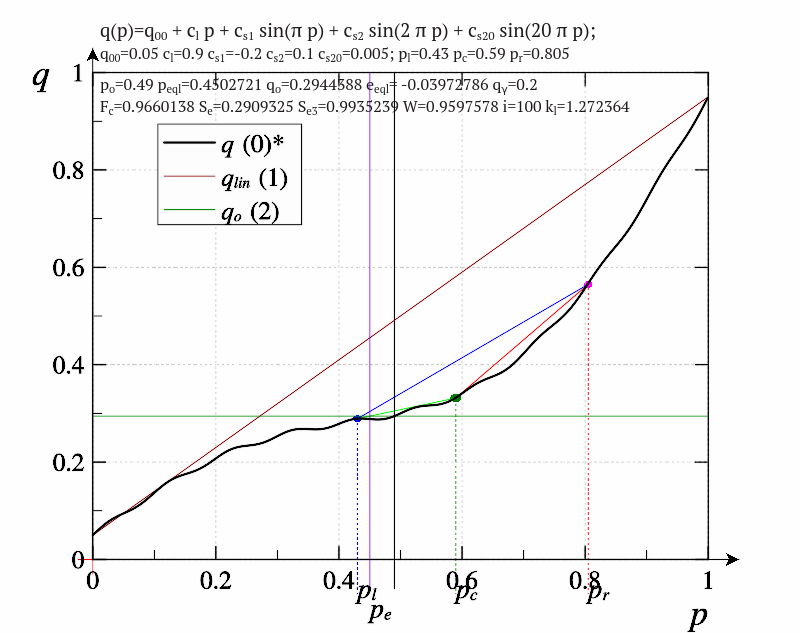
\includegraphics[width=49\TW]{p3/p/pq_sin-p_pq_po=049.png}
    \hfill
    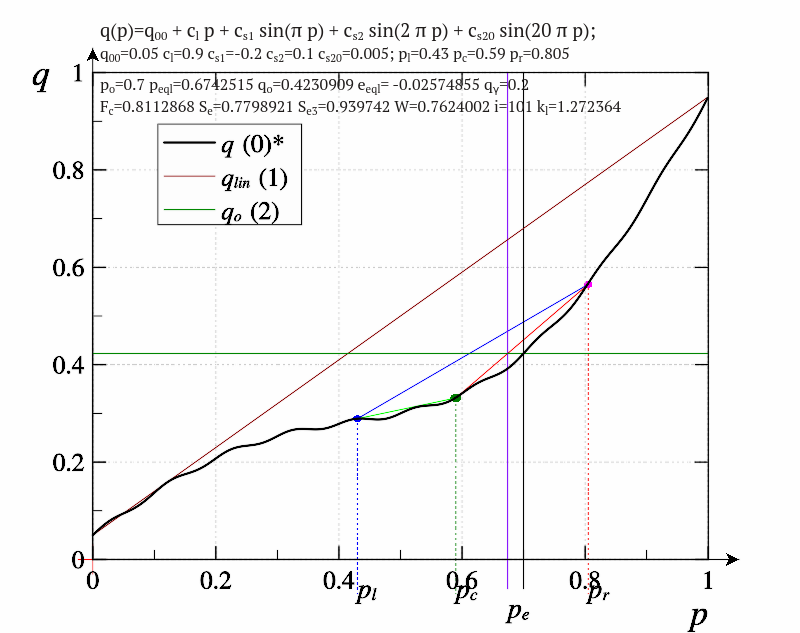
\includegraphics[width=49\TW]{p3/p/pq_sin-p_pq_po=070.png}
  }
  \caption{Конфігурації точок, відповідні випадку, що розглядається}
  \label{atu:f:pq_4}
\end{figure}

У цьому, найсприятливішому випадку проводиться інтерполяція, а не екстраполяція
залежності $ q(p)$, і досить вибрати ту ділянку, на якому гарантовано
відбувається перетин. При цьому значення всіх коефіцієнти підкреслюють
впевненість агента в значенні $ p_e $, що отримано:
%
\begin{equation}
  \tilde{p}_e
  =
  \begin{cases}
    \tilde{p}_{el}, & \tilde{q}_l < 0
    \\
    \tilde{p}_{er}, & \text{ otherwise}.
  \end{cases}
  ,
  c_\mathrm{su} = 1.0, \;  c_\mathrm{dist} = 0.5,  \;
  p_b =
  \begin{cases}
    -\tilde{p}_l, & \tilde{q}_l < 0
    \\
    \tilde{p}_r, & \text{ otherwise}.
  \end{cases}.
  \label{atu:eq:pr_e4}
\end{equation}

Останні випадки, за винятком точного збігу $q_o$ з $q_c$,
характерізуються меньшою ``упевненістю'' в отриманному значенню $p_e$,
що відображаєтся у коефіциентах 
$c_\mathrm{su}$, $\mathrm{dist}$ та  $p_b$.

У будь-якому з розглянутих випадків, має сенс ввести додаткове обмеження на
значення $ p_e $, так як через помилки вимірювання і моделювання воно може
виявитися навіть поза діапазону $ [p_{\min}, p_{\max}] $. З практичної
точки зору досить добре зарекомендувало себе обмеження
$ \tilde {p}_r \in [2 \tilde{p}_l, 2 \tilde{p}_r] $.
З урахуванням низького значення $ S $ для
агентів, які потрапили під таке обмеження, їх вплив на загальний результат буде
мінімальним, так як нормальному перебігу процесу ідентифікації існує хоча б
один агент з високим значенням $ S $. Більш суворі обмеження досить рідко
виправдовують себе, так як при цьому не використовуються екстраполяційні
властивості агентів.
Описаний даними правилами спосіб визначення $ p_e $ в подальшому будемо
означати як $p_{eql} $\label{atu:d:p_eql}.

% TODO: k_l ???

Розглянемо методи агентів, які Використовують значення функції якості. Єдиний
нерухомий агент, який використовує значення функції якості, ще більш марний (з
точки зору синтезу системи ідентифікації), ніж один нерухомий агент, який
використовує значення критерію.
У найпростіших випадках можлива побудова системи ідентифікації з однією моделлю
і, відповідно, одним пошуковим агентом.
Пара агентів, що взаємодіє між собою, здатна оцінити градієнт функції якості,
і, отже, забезпечити зміщення в потрібному напрямку.

Кожен пошуковий агент, визначаючи величину $ q_ {i} (t) $, і отримуючи $ q_o(t) $,
обчислює безрозмірну функцію якості ідентифікації $ F (q_o, q_i) $. Як
варіант, агент (або навіть вся керована частина системи ідентифікації) не має
безпосереднього доступу до критерію, і отримує власне значення~$F$.

Три сусідніх агента, взаємодіючі між собою, здатні не тільки оцінити градієнт
функції якості у своїй околиці, а й визначити (знову ж, оціночно) наявність там
максимуму.

На відміну від методів, які використовують значення критерію безпосередньо, в
цьому випадку немає можливості обробляти кожну з пар точок ($ p_l, p_c $) і ($
p_c, p_r $) незалежно. З трьох точок поблизу $ M_ {i} $ функція $ F (p) $
апроксимується параболою, і абсциса її вершини задає шукане значення параметра.
Змістимо початок координат в точку
$ ( p_c, F_c ) $. Тоді
%
\[
  \tilde{p}_c = 0, \,
  \tilde{p}_l = p_l - p_c, \,
  \tilde{p}_r = p_r - p_c.
\]
%
\[
  \tilde{F}_c = 0, \,
  \tilde{F}_l = F_l - F_c, \,
  \tilde{F}_r = F_r - F_c.
\]
%
\[
  \left\{
    \begin{array}{l}
      a_2 \tilde{p}_l^2 + a_1 \tilde{p}_l  = \tilde{F}_l
      \\
      a_2 \tilde{p}_r^2 + a_1 \tilde{p}_r  = \tilde{F}_r
    \end{array}
  \right. .
\]
%
\[
  a_1 = \frac{\tilde{F}_r \tilde{p}_l^2 - \tilde{F}_l \tilde{p}_r^2 }
             { \tilde{p}_l^2 \tilde{p}_r  - \tilde{p}_l \tilde{p}_r^2 }.
\]
%
\[
  a_2 = - \frac{\tilde{F}_r \tilde{p}_l - \tilde{F}_l \tilde{p}_r }
               { \tilde{p}_l^2 \tilde{p}_r  - \tilde{p}_l \tilde{p}_r^2 }.
\]

\begin{equation}
  \tilde{p}_e = - \frac{a_1}{2 a_2};
  \;
  p_e = p_c - \frac{a_1}{2 a_2}.
  \label{atu:eq:p_eFq}
\end{equation}

При цьому, якщо
$ a_2 \ge 0 $,
то потібне обмеження $p_e$ та корекція $c_\mathrm{su}$ та $c_\mathrm{dist}$.

Визначення $ p_e $ по (\ref{atu:eq:p_eFq}) будемо позначати як $p_{eFq}$.

Метод в найбільш сприятливому випадку, коли
$p_o \in [p_l,p_r]$, представлено на рис.~\ref{atu:f:p_eFq_intra}.

\begin{figure}[htb!]
  \centerline{
    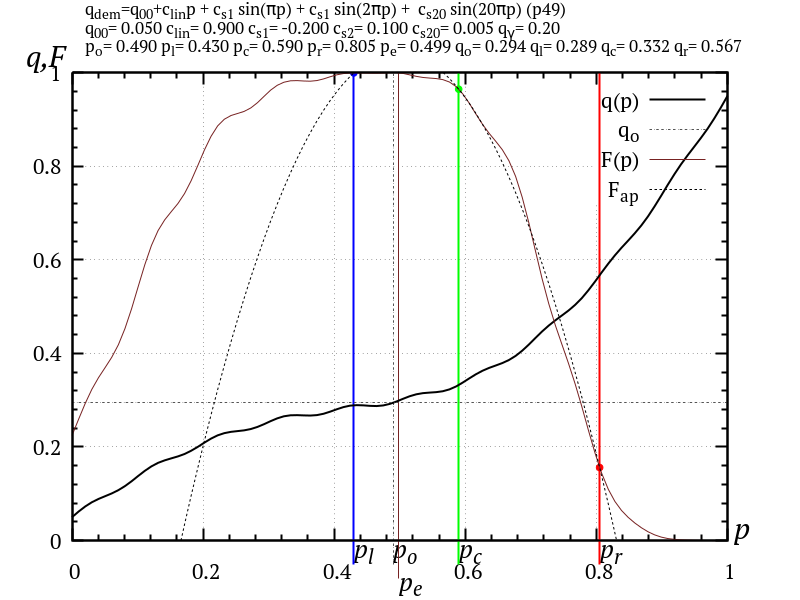
\includegraphics[width=49\TW]{p3/p/p_eFq/q_p_eFq_p49.png}
    \hfill
    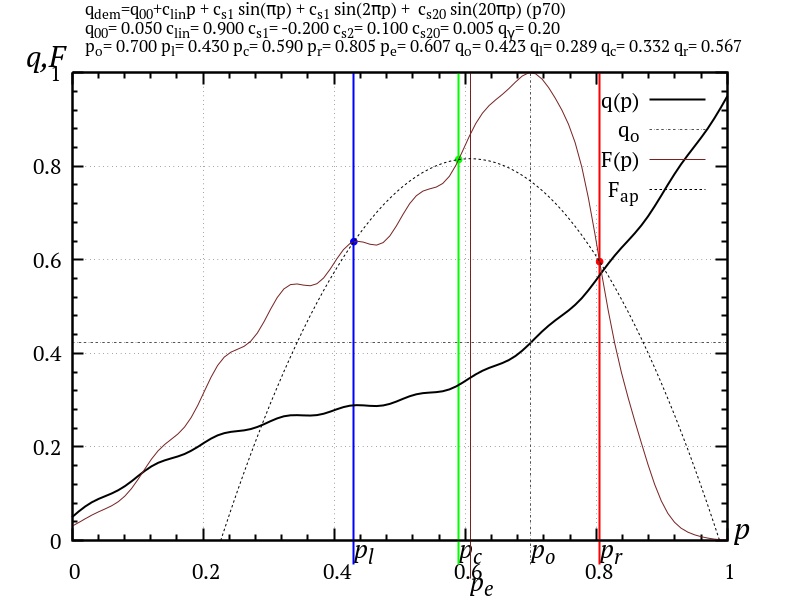
\includegraphics[width=49\TW]{p3/p/p_eFq/q_p_eFq_p70.png}
  }
  \caption{Визначення точки $ p_e $ методом $ p_{eFq} $ при $p_o \in [p_l, p_r] $}
  \label{atu:f:p_eFq_intra}
\end{figure}

Як і слід було очікувати, оцінка $ p_e $ в цьому випадку цілком спроможна, не
дивлячись на те, що в подібних умовах спостерігається різний рівень помилки
ідентифікації.

Цій метод демонструє суттєву чутлівість до значення $q_\gamma$.
Надлишкова чутливість призводить до того, що функція якості відмінна від нуля в
дуже вузькому діапазоні значень параметра, що призводить до практичної
безглуздості використовуваної апроксимації, і неадекватним результатами
ідентифікації.
Досить дивним є той факт, що при значному зменшенні чутливості помилка
ідентифікації росте дуже слабо. В першу чергу це пов'язано з тим, що в цих
умовах сама апроксимація кривої Гаусса параболою стає більш точною. Для інших
видів функції якості це не так. Більш того, наведені приклади розраховувалися
за умови відсутності помилок вимірювання. При недостатній чутливості
$ F_l \approx F_c \approx F_r \approx 1 $, і малі зміни $ F $ приведуть до значної
помилку ідентифікації.
В цілому, на підставі отриманих результатів, можна даний метод демонструє дещо
гірші результати, ніж $ p_{eql} $.

Досить простим і маловитратними з точки зору обчислень є метод оцінювання $ p_e $ методом
COG ( `` Center of gravity '') за значеннями функції якості:
%
\begin{equation}
  p_e =
  \frac{p_l F_l + p_c F_c + p_r F_r}{ F_r + F_c + F_r}  .
  \label{atu:eq:p_eFc}
\end{equation}

Умова обмеженості оцінки $ p_e \ in [p_l; p_r] $ в цьому випадку виконується
автоматично. Єдина складність --- обробка особливого випадку для тих видів $ F
(q) $, які звертаються в нуль на видаленні від центральної точки. В цьому
випадку знаменник (\ref{atu:eq:p_eFc}) звертається в нуль, в як $ p_e $ має
сенс вибрати $ p_c $. Для тих видів функцій якості, які не приймають строго
нульових значень, формально такої проблеми немає.  Для цього способу не представляється
можливим досить корисним способом визначити величину $ S $, тому, для
збереження однаковості покладемо $ S = 1 $.
Визначення $ p_e $ по (\ref{atu:eq:p_eFc}) в подальшому будемо позначати $p_{eFc}$.

Для визначення працездатності і властивостей різних методів оцінювання $ p_e $
в контрольованих умовах без урахування динаміки агентів, була обрана наступна
тестова задача: залежність $ q (p) $ визначалася по (\ref{atu:eq:q_dem}),
$p_{\min}=20$, $p_{\max}=60$,
$q_{00}=7$, $c_\mathrm{lin}=-4.0$.
Початкове розташування агентів рівномірний, і штучно зафіксоване:
$p_l=30$, $p_c=40$,  $p_r=50$.

У першій серії обчислювальних експериментів значення параметра об'єкта $ p_o $
змінювалося в діапазоні $ [p_ {\min}; p_{\max}] $ при фіксованій відстані
між агентами $ A = p_c - p_l = p_r - p_c $. Це дозволило оцінити як
інтерполяційні (при $ p_o \in [p_l, p_r] $), так і екстраполяційні можливості
методів. Так як частина методів при визначенні $ p_e $ використовує значення
функції якості, то при проведенні експериментів величина $ q_\gamma $ також
варіювалася.

На рис.~\ref{atu:f:qsl_pe_po_qg_all} представлені залежності помилок
ідентифікації для тестового завдання (\ref{atu:eq:q_dem}) при повному
комплекті нелінійних членів  трьома нерухомими
агентами трьома розглянутим методами визначення $ p_e $.

\begin{figure}[htb!]
  \centerline{
    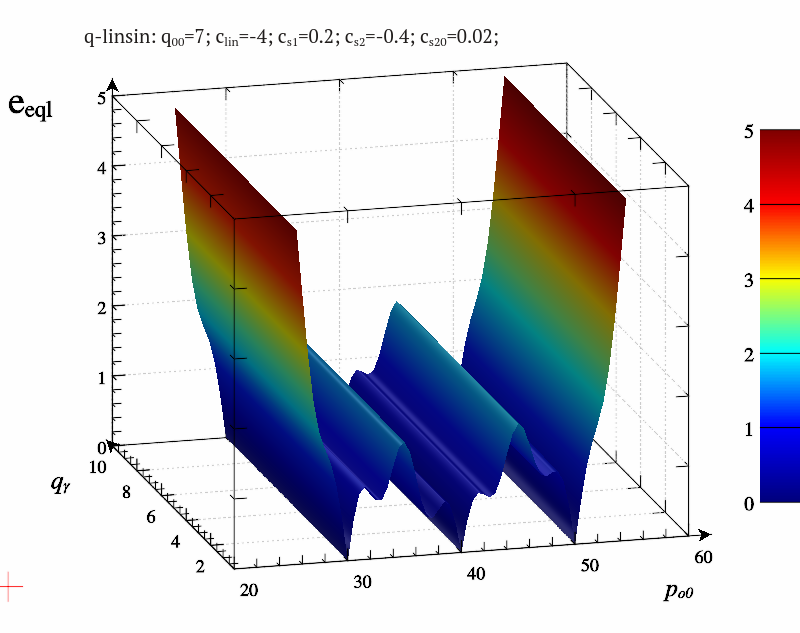
\includegraphics[width=0.32\textwidth]{p3/p/qls_pe-p_po_qg_eql_all.png}
    \hfill
    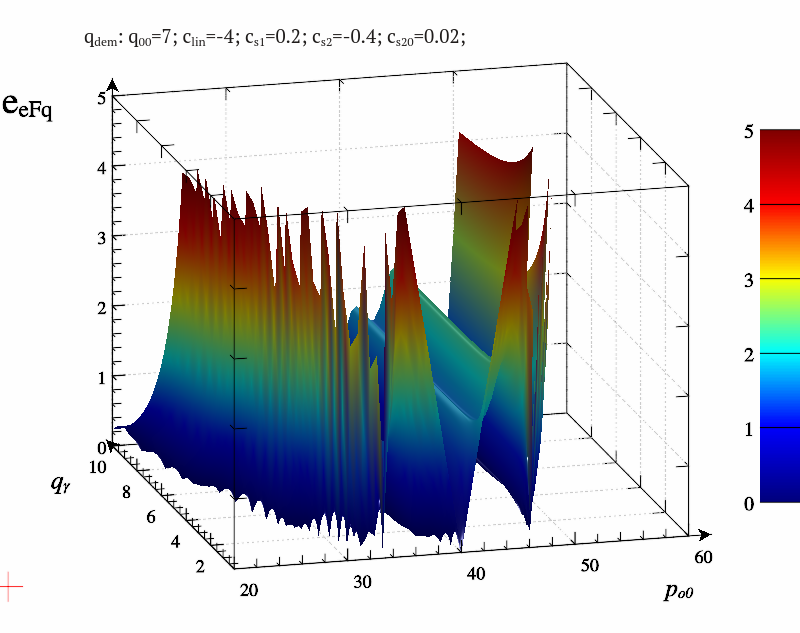
\includegraphics[width=0.32\textwidth]{p3/p/qls_pe-p_po_qg_eFq_all.png}
    \hfill
    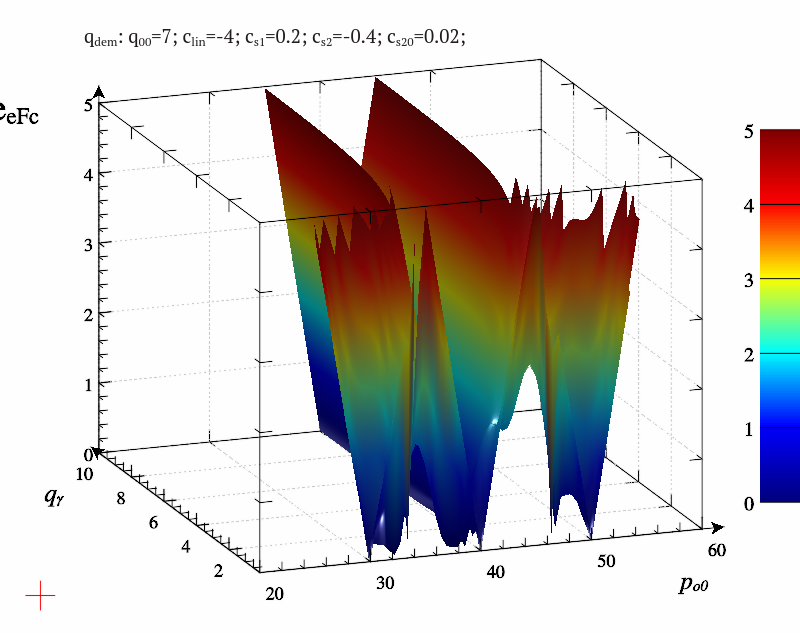
\includegraphics[width=0.32\textwidth]{p3/p/qls_pe-p_po_qg_eFc_all.png}
  }
  \caption{Залежності $e(p_o,q_\gamma)$ для методов $p_{eql}$, $p_{eFq}$, $p_{qFc}$ при повному комплекті нелінійних членів}
  \label{atu:f:qsl_pe_po_qg_all}
\end{figure}

Метод $ p_ {eql} $ демонструє досить обмежену помилку ідентифікації при
$ p_o \in [p_l; p_r] $, і досить швидкий, але лінійно обмежений зростання помилки за
межами цього робочого діапазону. Метод $ p_{eFq} $ виявляє істотну залежність
від величини $ q_\gamma $: малі значення призводять до суттєвого
зростання помилки, а з подальшим зростанням рівень помилки в межах робочого
діапазону приблизно одного порядку з помилкою в методі $ p_{eql} $. При
цьому, за межами робочого діапазону спостерігається більш суттєве зростання
помилки. Метод $ p_ {qFc} $ демонструє прийнятні результати тільки в дуже
вузькому діапазоні значень $ q_\gamma $, що ставить під серйозний сумнів
можливість застосування цього методу для реальних завдань, так як при цьому
немає можливості передбачити то значення цього параметра, при якому метод буде
працездатний.

На рис.~\ref{atu:f:qsl_S_po_qg_all} представлені залежності
$ S (p_o, q_\gamma) $
при тих же умовах, при яких було отримано рис.~\ref{atu:f:qsl_pe_po_qg_all}.
Використовувалося визначення (\ref{atu:eq:S3}), як
потенційно більш адекватне помилку ідентифікації.

\begin{figure}[htb!]
  \centerline{
    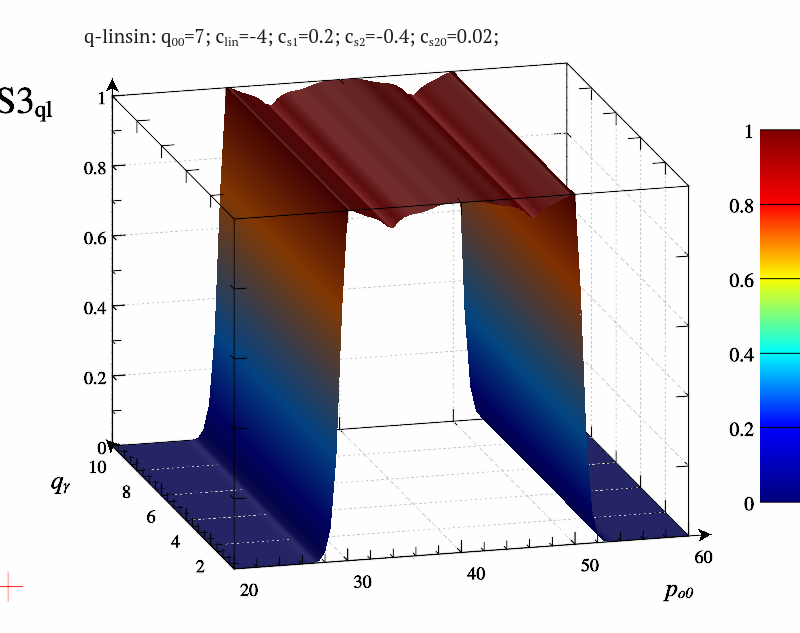
\includegraphics[width=0.32\textwidth]{p3/p/qls_pe-p_po_qg_Sql_all.png}
    \hfill
    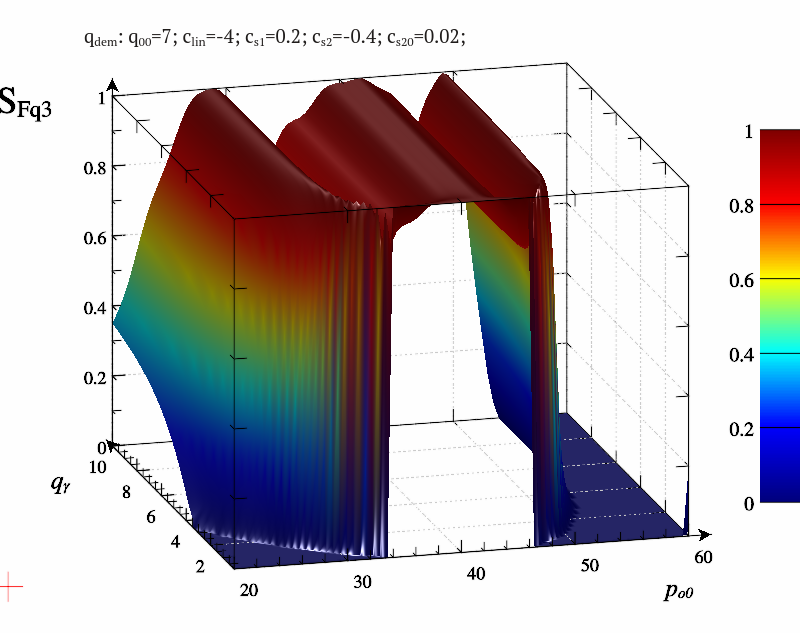
\includegraphics[width=0.32\textwidth]{p3/p/qls_pe-p_po_qg_SFq_all.png}
    \hfill
    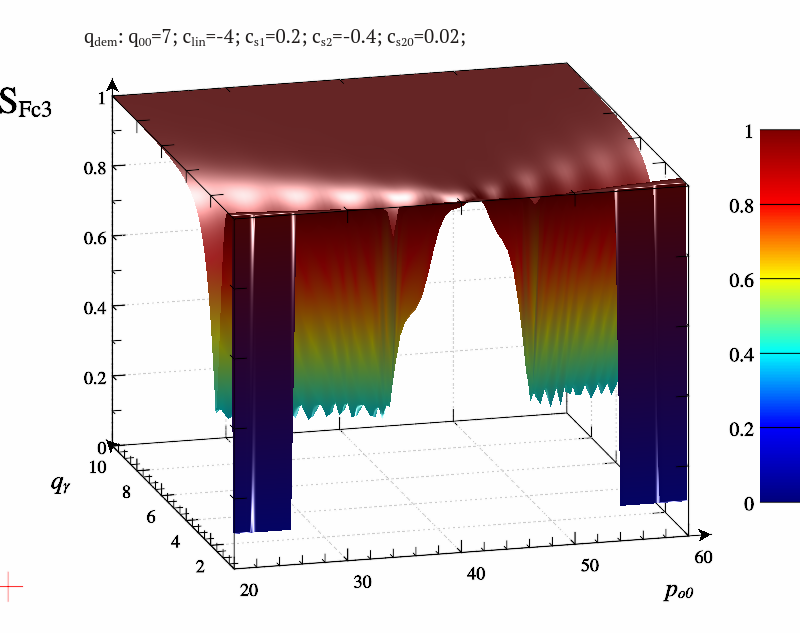
\includegraphics[width=0.32\textwidth]{p3/p/qls_pe-p_po_qg_SFc_all.png}
  }
  \caption{Залежності $S(p_o,q_\gamma)$ для методів $p_{eql}$, $p_{eFq}$, $p_{qFc}$}
  \label{atu:f:qsl_S_po_qg_all}
\end{figure}

Для методу $ p_{eql} $ близькі до одиниці значення $ S $, як і планувалося,
спостерігаються в тих же областях, де і низький рівень помилки ідентифікації, в
першу чергу --- всередині робочого діапазону. При цьому, ця величина не
повторює рівень помилки, так як це неможливо визначити за трьома точкам. Метод
$ p_ {eFq} $ також характеризується досить осмисленим видом цієї залежності,
включаючи низький рівень впевненості при підвищеній чутливості функції якості.
Навпаки, для методу $ p_ {eFc} $ графік показує, що для нього це визначення $ S$ не має сенсу.

У другій серії обчислювальних експериментів значення параметра об'єкта було
фіксованим $ p_o = 39 $, а відстань між агентами $ A $ змінювалося від $ 0.1 $
до $ 20 $. При цьому, при $ A <1 $ точка $ p_o $ перебувала за межами інтервалу
$ [p_l, p_r] $, і становище $ p_e $ визначалося за допомогою екстраполяції.
Значна частина цих графіків відображає протилежний випадок --- $ p_O \in [p_l,p_r] $,
і значення $ p_e $ визначається інтерполяцією на розширенні (з ростом $A $) діапазоні.
На рис.~\ref{atu:f:qsl_pe_A_qg_all} представлені поверхні залежно помилок ідентифікації
при наявності всіх нелінійних членів.

\begin{figure}[htb!]
  \centerline{
    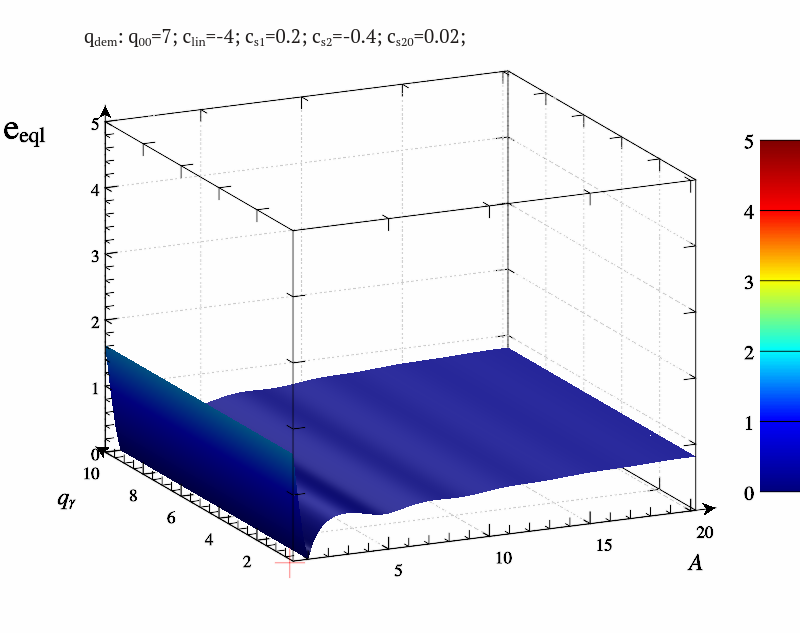
\includegraphics[width=0.32\textwidth]{p3/p/qls_pe-p_A_qg_eql_all.png}
    \hfill
    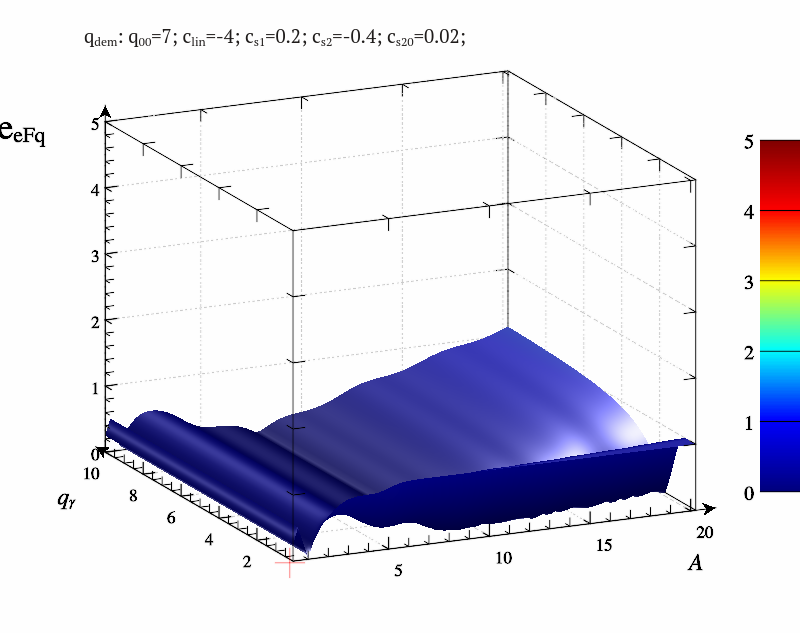
\includegraphics[width=0.32\textwidth]{p3/p/qls_pe-p_A_qg_eFq_all.png}
    \hfill
    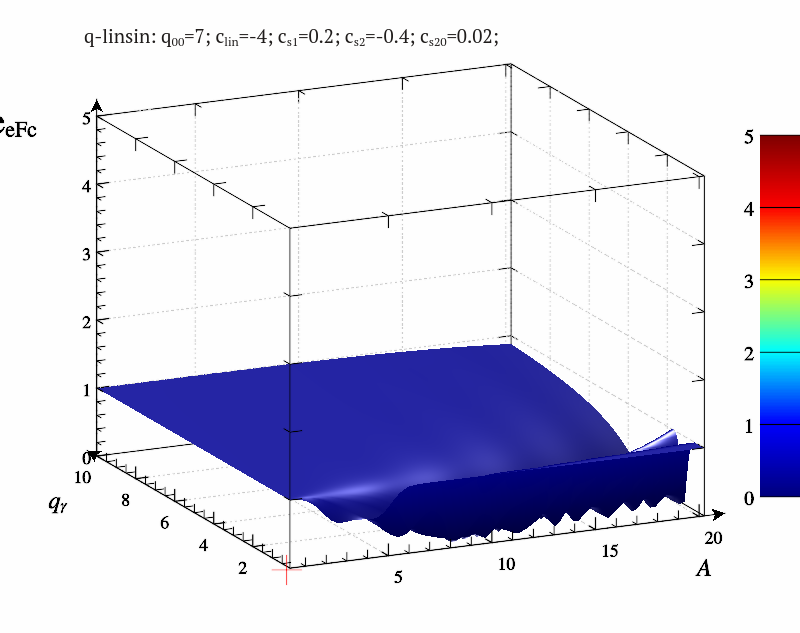
\includegraphics[width=0.32\textwidth]{p3/p/qls_pe-p_A_qg_eFc_all.png}
  }
  \caption{Залежності $e(A,q_\gamma)$ для методов $p_{eql}$, $p_{eFq}$, $p_{qFc}$}
  \label{atu:f:qsl_pe_A_qg_all}
\end{figure}

Для методу $ p_{eql} $ форма цього графіка досить передбачувана --- немає
залежності від $ q_\gamma $, на ділянці екстраполяції величина помилки
лінійно падає при $ A \to p_c - p_o $. При подальшому зростанні $ A $ помилка
помірно зростає, причому в цьому зростанні можна виділити дві ділянки. Перший
характеризується відносно різким зростанням помилки, пов'язаних зі збільшенням
вплив високочастотних нелінійних членів, другий --- досить плавним підйомом.
Графік, відповідний методу $ p_{eFq} $ проявляє явну залежність помилки від
$q_\gamma$. Для широкого діапазону величини $ A $ існує досить вузька область
значень $ q_\gamma $, при яких помилка мінімальна. Як надмірна, так і
недостатня чутливість функції якості призводить до зростання помилки.
Графік помилки для методу $ p_{eFc} $ підкреслює обмежену придатність цього методу.

Таким чином, на підставі результатів моделювання можна зробити висновки про
можливість застосування розглянутих методів. Метод $ p_{eFc} $ має гранично
обмежену придатність, подальших дослідженнях в даній цей метод застосовуватися
не буде. При нормальному функціонуванні метод $ p_{eql} $ забезпечує найкращі
результати. При цьому він складніше в реалізації, вимагає обробки ряду
особливих випадків. Метод $ p_{eFq} $ демонструє результати, які можна
порівняти з методом $ p_ {eql} $, при цьому він простіше в реалізації. У тих
випадках, коли величина критерію самому агенту безпосередньо не відома, цей
метод, на відміну від методів, заснованих і апроксимації $ q (p) $, зберігає
працездатність. Недоліком є істотна залежність від величини $ q_\gamma $.
Методи $ p_ {eql} $ і $ p_ {qFq} $ дозволяє досягти меншої помилки
ідентифікації при зближенні пошукових агентів до $ p_o $, за умови $ p_o \in [p_l, p_r] $.


% {Динамика поисковых агентов}

Значення $ p_e $, отримане пошуковим агентом, може використовуватися
безпосередньо і миттєво в якості значення параметрів для керованих моделей
тільки в тому випадку, якщо об'єкт, і отже моделі, не виявляють власної
динаміки, тобто є статичними. Ідентифікація статичних об'єктів не є завданням в
даній роботі.

При моделюванні динаміки тіла без урахування обертання в механіці досить задати
всі сили, що діють на це тіло. Аналогічно, визначаючи пошукову динаміку агента
потрібно визначити еквівалент ``сил'', що викликають зсув параметрів моделей,
контрольованих агентом. При цьому завдання визначення динаміки можна спростити,
розділивши ``сили'' на дві групи. До першої входять сили, що призводять до ``руху''.
У другу входять сили опору, і замість розгляду самих сил досить
визначити правила динаміки, при цьому можливе використання правил, які не мають
прямого відображення на реальні фізичні системи.

Розглянемо способи визначення основних діючих сил.

$f_e $ --- ``сила тяжіння'' до локальної оцінці $ p_e $, забезпечує зміщення
агента в напрямку цієї точки, і, отже, збільшення ``щільності'' агентів в
околицях $p_o$. Найпростішим, очевидним, з прозорим фізичним змістом є
наступне визначення:
%
\begin{equation}
  f_e(t) = - k_e \left( p_c(t) - p_e(t) \right)  ,
  \label{atu:eq:f_e_lin}
\end{equation}
%
де $ k_e $ --- коефіцієнт пропорційності, відповідний коефіцієнту жорсткості
умовної ``пружини'', що деформується при видаленні $ p_c $ від $ p_e $. Це
визначення досить універсально, і має сенс при реалізації багатьох пошукових
тактик. Розглянуто інши способи визначенния цієї сили, зокрема з фіксованою
абсолютною велчиной та змінним напрямком, то гібрідне визначення.
Загальним недоліком визначення сили $ f_e $ за виразом (\ref{atu:eq:f_e_lin})
є те, що сила визначається тільки по локальним параметрами в околиці
агента. Більш того, ігнорується навіть локальне значення впевненості агента в
оцінці $ p_e $. Тому має сенс використовувати додатковий множник у визначенні $f_e$,
наприклад $F$, $S$, $W$.

Наявність тільки сили $ f_e $ призводить до того, що поведінка агентів буде
практично незалежним, і для реалізації властивостей ``ансамблю'' агентів
необхідне введення сил, що регламентують колективна поведінка. В першу чергу,
слід визначити силу $f_n$, визначальну взаємодія агента з найближчими
сусідами. У досить загальному випадку цю силу можна визначити як
%
\begin{equation}
  f_n( p_r, p_c, p_l ) = f_{nr}(p_r-p_c) + f_{nl}(p_c-p_l).
  \label{atu:eq:f_n_gen}
\end{equation}

У разі лінійності і однакових визначень функцій $ f_ {nr} $ і $ f_ {nl} $ ця залежність набуває вигляду
%
\begin{equation}
  f_n = k_n ( p_r - 2 p_c + p_l ),
  \label{atu:eq:f_n_lin}
\end{equation}
%
де $ k_n $ --- масштабний коефіцієнт, що відповідає коефіцієнту жорсткості
``пружин'', що з'єднують агенти. При цьому слід зазначити, що ця функція буде
приймати нульові значення при будь-якому рівномірному розподілі агентів.
Для уникання цього недоліку, та запобігання перехресту траекторі агентів,
можна використати таке визначенния:
%
\begin{equation}
  f_n = k_n \left( \log\left( \frac{p_r-p_c}{p_{d0}} \right) -  \log\left( \frac{p_c-p_l}{p_{d0}}\right) \right),
  \label{atu:eq:f_n_log}
\end{equation}
%
где
$p_{d0}$ ---
базова відстань між агентами, звичайно дорівнює початкової віддалі.

Також має сенс використовувати $f_c$ --- ``силу тяжіння'' до початкового значення параметра
($ p_{c}(0) $) для даної моделі. У лінійній постановці ця сила визначається як
%
\begin{equation}
  f_c = -k_c (p_c - p_{c}(0)) ,
  \label{atu:eq:f_c}
\end{equation}
%
де $k_c$ --- коефіцієнт, що відповідає жорсткості ``пружини'',
що зв'язує агента з його початковим положенням.
Добре зарекомендували себе як нелінійні ``бар'єри'',
так і алгорітмічні методи, які утримують агента
більш-мень жорстко у виділеному йому диапазоні параметра.

З урахуванням вищевикладеного, визначимо суму всіх ``сил'',
що діють на пошуковий агент:
\begin{equation}
  f_t = f_c + f_n + f_e .
  \label{atu:eq:f_t}
\end{equation}


Можна використовувати різні способи визначення пошукової динаміки агента при
заданій силі. Наприклад, метод ``важкого кульки'':
\begin{equation}
  m \ddot{p}_c + \nu \dot{p}_c = f_t(t),
  \label{atu:eq:heavy_ball}
\end{equation}
%
де $ m $ --- еквівалент маси кульки, $\nu$ --- коефіцієнт умовної в'язкості.

Також може використовуватися прібліженіня динаміки тіла в в'язкої рідини, коли
вплив інерції дуже малий в порівнянні з в'язкістю, при цьому зміни параметрів
моделей (пошукових агентів) задається наступним чином:
%
\begin{equation}
  \od{p_c}{t} = v_f f_t(t),
  \label{atu:eq:v_f}
\end{equation}
%
\noindent
де $ f_t $ --- сума всіх діючих `` сил '',
$ v_f = 1 / \nu $ --- коефіцієнт
пропорційності. Даний підхід, в порівнянні з попереднім, вимагає менших
обчислювальних витрат, і проявляє більшу стійкість. Більш слабкі пошукові
здібності компенсуються застосуванням безлічі агентів. Тому, в подальшому
викладі для многомодельного систем буде застосовуються саме цей підхід.

Існують методи адаптивно-пошукової ідентифікації, що визначають свої правила опису пошукової динаміки.


Розглянемо набір підходів до визначення пошуковим координатором точки максимуму
функції якості, а отже --- значення ідентифікованого параметра
\cite{atu_st99,atu_jacs2015}.

Из всего списка выходных сигналов поисковых агентов координатор использует
только необходимое ему подмножество. В качестве координат может использоваться
как $p_c$, так и $p_e$. В качестве уровня важности может использоваться $F$,
$S$, $W$.

З усього списку вихідних сигналів пошукових агентів координатор використовує
тільки необхідне йому підмножина. Як координат може використовуватися як
$ p_c$, так і $ p_e $.
У якості рівня важливості може використовуватися $ F $, $ S $, $W$.
В якості першого наближення можна як $ p_\mathrm{id} $ використовувати
значення $ p_c $ тієї моделі, для якої функція якості максимальна:
%
\begin{equation}
  p_{bcF}
  =
  p_{c,i};
  \quad
  i : F_i = \max{F_j}, \, j=0 \ldots N-1 .
  \label{atu:eq:p_bcF}
\end{equation}

Аналогічно визначаються залежності
$p_{bcS}$ та $p_{bcW}$.
Єдиною перевагою даного методу є простота реалізації. При цьому, ніяк не
використовуються аппроксимирующие здатності агентів. Більш того, залежності
$ p_{bcA} (t) $ схильні до стрибкоподібним змінам в момент перемикання з однієї моделі
на іншу. Слід зазначити, що для методів, які використовують одну модель це
практично єдиний метод визначення
$p_\mathrm{id}(t)$.

Для того, що б використовувати аппроксимирующие можливості кожного агента, у
визначенні (\ref{atu:eq:p_bcF}) замість $ p_c $ можна використовувати $ p_e$.
Відповідні методи отримають позначення $ p_ {beS} $, $ p_ {beS} $ і $ p_{beW} $.
Такі визначення, на відміну від (\ref{atu:eq:p_bcF}) дозволяють,
при досить хорошій апроксимації $ q (p) $ принаймні одним кращим агентом,
реалізувати ідентифікацію для будь-якого
$ p_o \in [p_{\min} , p_{\max}]$ при нерухомих агентів.

Наступний метод --- реалізація методу COG (Center of gravity, Такагі-Сугено \cite{atu_asau25,atu_csit2015,atu_asau16},)
використовуваного при дефаззифікації систем нечіткої логіки для всього
ансамблю:
%
\begin{equation}
  p_{gcF}
  =
  \frac{\sum\limits_{i=0}^{N-1} F_{i} p_{i}}
       {\sum\limits_{i=0}^{N-1} F_{i} }
  .
  \label{atu:eq:p_gcF}
\end{equation}
%
Аналогічно визначаються методи
$p_{gcS}$,
$p_{gcW}$,
$p_{geF}$,
$p_{geS}$ та
$p_{geW}$.


Наступний підхід покликаний зменшити залежність першого від впливу локальних
екстремумів і кордонів. В цьому випадку визначається модель $ M_{i_{m}} $ ($ M_{c} $) з
максимальним значенням $ F $, а в оцінці використовується тільки найближча
околиця цієї моделі:
%
\begin{equation}
  p_{leF}
  =
  \frac{ F_{l} p_{l} + F_{c} p_{c} + F_{r} p_{r} }
       { F_{l}       + F_{c}       + F_{r}       }
  .
  \label{atu:eq:p_lcFl}
\end{equation}
%
Аналогічно визначаються методи
$p_{lcS}$,
$p_{lcW}$,
$p_{leF}$,
$p_{leS}$ та
$p_{leW}$.


Так само в околиці кращого агента можна використовувати інтерполяцію по
$ F $, аналогічно (\ref{atu:eq:p_eFq}). В позначенні таких методів будемо
використовувати перший символ ``q'', наприклад $ p_{qeF}$.

Помилки ідентифікації в просторі параметрів для розглянутих підходів позначимо відповідно:
%
\begin{equation}
  e_{gcF} = p_{gcF} - p_o,
  \quad
  e_{leF} = p_{leF} - p_o,
  \quad
  \ldots
  \quad
  e_{leW} = p_{leW} - p_o.
  \label{atu:eq:e_xx}
\end{equation}
%

У даній роботі розглядається набір методів ідентифікації нелінійних динамічних
систем. При цьому, більшість з них мають загальні властивості, і система
ідентифікації в цілому складається з ``набору'' модулів і алгоритмів,
комбінація яких дозволяють вибрати конкретний метод, що підходить для даної
задачі.
Пропонується до використання наступна система позначень, послідовно визначає
компоненти системи ідентифікації, починаючи з агентів.

\begin{enumerate}

  \item
  Перший символ (``F'', ``q'', ``x'' ) визначає,
  яка величина використовується кожним агентом для визначення $ p_e $.

  \item

    Другий символ (``l'' --- linear, ``q'' --- quadratic \ldots ) задає спосіб визначення величини $ p_e $ одним агентом.

  \item
  Третій символ визначає локальну пошукову геометрію, найчастіше --- кількість
    агентів в в пошуковій групі, наприклад: ``2'' --- пошукова пара, ``3'' --- триплет.

  \item
    Четвертий символ (``z'' --- zero, ``r'' --- real \ldots),
    описує поведінку додаткових моделей, які перебувають на кордоні:

  \item
    П'ятий символ (``c'' --- const, ``l'' --- linear \ldots )
    позначає вибрану залежність для величини $ f_e $ (або
    аналогічної величини, якщо $ f_e $ безпосередньо не використовується).

  \item
    Шостий символ (``o'' --- one, ``F'', ``S'', ``W'') визначає множник,
    використовуваний для величини $ f_e $ при визначенні динаміки об'єкта.

  \item
   Сьомий символ (``z'' --- zero, ``v'' --- viscous \ldots)
    вказує, яким чином величина $ f_t $ (або її еквівалент) впливає на динаміку агента.

  \item
   Восьмий (``n'' --- none, ``t'' --- triangle \ldots ) символ дозволяє вказати, яке додаткове пошуковий рух реалізує агент.

  \item
    Дев'ятий символ задає спосіб визначення ідентифікованого параметра по всьому ансамблю:
    \begin{description}

      \item[b]  --- ``best''
        --- вибирається найкращий агент без подальшої обробки;

      \item[g]  --- ``global COG'' ---
        метод ``Center of Gravity'' по всьому ансамблю~(\ref{atu:eq:p_gcF});

      \item[l] --- ``local COG'' ---
        метод ``Center of Gravity'' по околиці кращого агента;

      \item[q] ---
        інтерполяція другого порядку в околиці кращого агента~(\ref{atu:eq:p_eFq}).

    \end{description}

  \item
    Десятий символ (``c'', ``e'') визначає, який з вихідних сигналів пошукового агента використовується.

  \item
    Одинадцятий символ (``F'', ``S'', ``W'') вказує, яка величина використовується для завдання ваги кожного агента.


\end{enumerate}
%
Для позначення підмножин методів замість позначення елемента використовується символ ``A'' --- ``any''.
Якщо виникає потреба вказати конкретний вид критерію, то в кінець даного
позначення, через точку, додається позначення використовуваного критерію.

Приклад позначень:
``Fc3zlovngcW.$q_{x^2}$''
--- метод, агенти якого для оцінювання величини $ p_e $ використовують функцію
якості і квадратичну апроксимацію за даними кожних трьох сусідніх агентів, 2
псевдомоделі на кордоні, залежність $ f_e (p_e-p_c) $ --- лінійна, ``в'язка''
динаміка, одиничний коефіцієнт при цій силі, ``global COG'' для результуючого
значення параметра по значенням $p_c$ і $W$, критерій
``$q_{x^2}$''.


Якість ідентифікації для процесу в цілому задається мірою:
%
\[
  \overline{e} = \mu( p_o(t), p_\mathrm{id}(t) ),
  \quad
  t \in [0;T].
\]

Конкретний вид міри визначається завданням. Якщо в конкретній постановці
важливо знати максимальне відхилення ідентифікованого параметра моделі від
об'єкта, то має сенс вибрати міру $ C[0; T] $ або ж $ R_{\infty}^n$ для
дискретного представлення:
%
\begin{equation}
  \overline{e_c}(p_o(t),p_\mathrm{id}(t))
  =
  \max \big| p_o(t)-p_\mathrm{id}(t) \big|,
  \quad
  t \in [0;T].
  \label{atu:eq:e_c}
\end{equation}

Більш поширеним є випадок, коли інтерес представляє не максимальне значення
$ |e(t)| $, а якийсь варіант усереднення цієї величини, наприклад
%
\begin{equation}
  \overline{e_2}(p_o(t),p_\mathrm{id}(t))
  =
  \sqrt{ \frac{1}{T} \int\limits_{0}^{T} \big( p_o(t)-p_\mathrm{id}(t) \big)^2 \, \mathrm{d}t },
  \label{atu:eq:e_2}
\end{equation}

Саме значення як помилки ідентифікації, так і відповідноі міри ---
величина розмірна, і в такому вигляді не придатне для незалежного від
конкретної ситуації оцінювання якості роботи методу. Розглянемо можливі
величини, що дають можливість привести помилку ідентифікації до безрозмірного
вигляду. В першу чергу, припустимо, що взагалі не проводимо ніякої
ідентифікації, а в якості значення параметра використовуємо або геометричний
центр $ p_{00} $ безлічі $ \mathcal{P} $, або, якщо це з якої-небудь причини
відомо, точку з максимальним значенням щільності ймовірності. тоді позначимо
%
\begin{equation}
  \overline{e}_{00}
  =
  \overline{e}(p_o(t),p_{00})
  \label{atu:eq:e_00}
\end{equation}

Відносні помилки для відповідних абсолютних~(\ref{atu:eq:e_xx})
тоді будуть визначені в такий спосіб:
%
\begin{equation}
  \overline{e}_{rbcF} = \frac{\overline{e}_{bcF}}{\overline{e}_{00}}, \;
  \overline{e}_{rleS} = \frac{\overline{e}_{leS}}{\overline{e}_{00}}, \;
  \overline{e}_{rgeW} = \frac{\overline{e}_{geW}}{\overline{e}_{00}},
  \ldots
  \overline{e}_{rqeF} = \frac{\overline{e}_{qeF}}{\overline{e}_{00}}.
  \label{atu:eq:e_rxx}
\end{equation}

Близькість цих величин до одиниці свідчить про те, що даний метод ідентифікації
в розглянутих умовах марний. Більш того, при серйозних порушеннях в процесі
пошуку, наприклад при втраті стійкості, ці величини можуть і перевершувати
одиницю. Використовуються також методи обезразмеріванія, що враховують
використання декількох агентів.

Дослідження працездатності та властивостей методів на тестових завданнях.

Для оцінювання можливостей системи ідентифікації відстежувати як гладкі, так і
стрибкоподібне зміни параметрів, пропонується для кожної тестової системи, якщо
це можливо, проводити моделювання процесів ідентифікації за умови, що зміна
значення параметра об'єкта описується одним з наступних виразів:
%
\begin{equation}
  p_o(t) = p_0 +  U_{p} \sign \sin( \omega_{p} t ),
  \label{atu:eq:po_t_sign}
\end{equation}
%
%
\begin{equation}
  p_o(t) = p_0 +  U_{p} \sin( \omega_{p} t ).
  \label{atu:eq:po_t_sin}
\end{equation}
%
\begin{equation}
  p_o(t) = p_0 +  U_{p} \frac{t}{T}.
  \label{atu:eq:po_t_ramp}
\end{equation}


Розглянемо конфігурації рівноважного стану пошукових агентів при застосуванні
різних пошукових тактик з числа розглянутих. Для даного завдання немає
необхідності розглядати поведінку координатора пошуку, тому три правих символу
класифікації тут значення не мають.
Використовувалося 5 пошукових агентів: $ A_0 \ldots A_4 $, початкові
координати яких ($ p_ {ci,0} $) були розподілені по пошуковому діапазони
рівномірно. Залежність $ p_o (t) $ задана як (\ref{atu:eq:po_t_ramp}), при
цьому величини $ p_o $ і $ U_p $ обрані таки чином, щоб покрити весь робочий
діапазон: $ p_0 = p_{c0,0} = 20 $, $ U_p = p_ {c4,0} - p_ {c0,0} = 40 $.


На рис.~\ref{atu:f:qls_ramp_Fq3rlovnAAF} наведені результати моделювання при використанні групи методів
``Fq3rlovnAAF''. Слід зазначити, що практично у всьому діапазоні об'єкт
``супроводжується'' двома агентами, і тільки в області ``передачі'' наступній
групи це число зростає до трьох. Слід зазначити відсутність коливань. До
негативних явищ можна буде назвати те, що далекі агенти притискаються до
кордону виділеної їм області, що викликано використанням одиничного множника у
визначенні $ f_e $. Також необхідно відзначити збільшення
``дистанції супроводу'' в околиці точки $ p_o = 40 $, $ t = 10 $.

\begin{figure}[htb!]
  \centerline{
    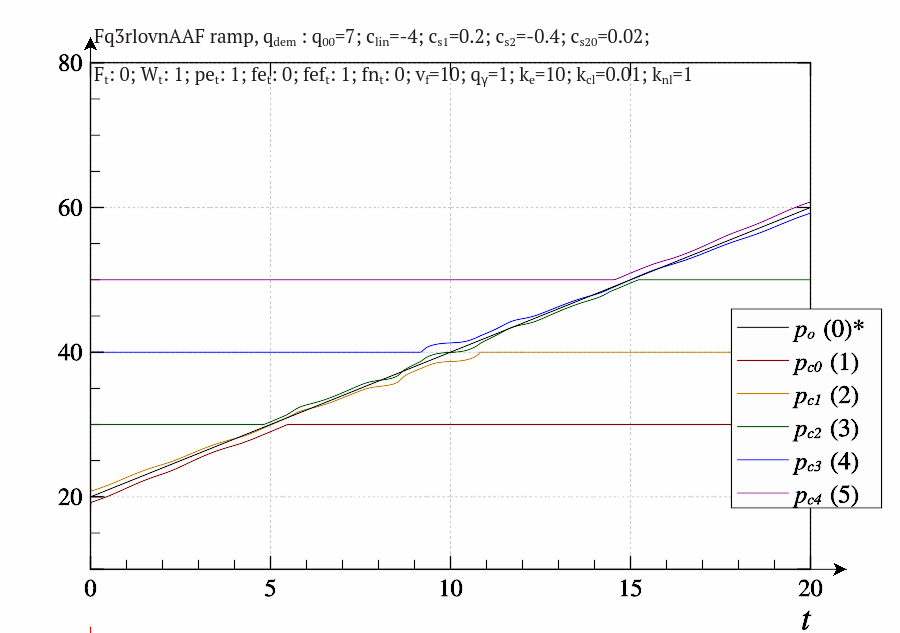
\includegraphics[width=0.70\textwidth]{p3/p/ramp/qls-p_t_pi_Fq3rlovnAAF_ramp.png}
  }
  \caption{Рівноважні конфігурації агентів при використанні группи методів  Fq3rlovnAAF}
  \label{atu:f:qls_ramp_Fq3rlovnAAF}
\end{figure}

На рис.~\ref{atu:f:qls_ramp_Fq3rlovnAAF} наведені результати моделювання при використанні групи методів
``ql3rlWvnAAF''.
Відмінність проявляється в меншому зміщенні віддалених агентів, що, без
істотної зміни точності повинно призводити до зменшення часу реакції системи на
стрибкоподібне зміна параметра.

\begin{figure}[htb!]
  \centerline{
    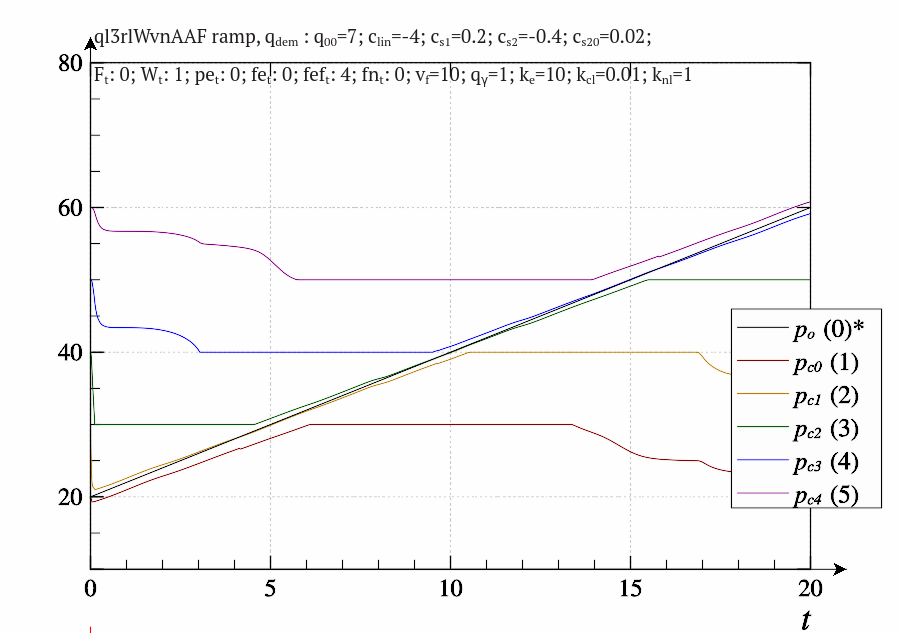
\includegraphics[width=0.70\textwidth]{p3/p/ramp/qls-p_t_pi_ql3rlWvnAAF_ramp.png}
  }
  \caption{Рівноважні конфігурації агентів при використанні группи методів ql3rlWvnAAF}
  \label{atu:f:qls_ramp_ql3rlWvnAAF}
\end{figure}


Також булу досліджено рівновіжні конфігурації агентів для
групп методів
``Fq3rlFvnAAF'',
``Fq3rlSvnAAF'',
``Fq3rlWvnAAF'',
``ql3rlovnAAF'',
``ql3rlFvnAAF'' та
``ql3rlSvnAAF''.
Встановлено, що в тих випадках, коли для оцінювання $ p_e $ використовується
метод $ p_{eFq} $, то не має сенсу в якості множника при $ f_e $
використовувати $ S $ або $ W $. Найкращим вибором в цих умовах будует
використання значення функції якості $ F $. До того ж, що підтверджується і
результатами дослідження якості апроксимації $ q (p) $, використання методів,
які використовують кусково-лінійну апроксимацію, найбільш прийнятний. У цих
умовах стає виправданим як вищезгаданого множника використовувати
$ S $ і $ W$, причому останній варіант видається більш виправданим.


Рівноважні конфігурації агентів, представлені вище, дають інформацію тільки про
потенційних якостях систем ідентифікації. В першу чергу, якість визначається
помилкою ідентифікації. В якості тестової задачі
використовується~(\ref{atu:eq:q_dem}) з усіма нелінійними членами. При цьому для кожного методу
проводилася серія обчислювальних експериментів з різним значенням $ p_o $. Інші
параметри як системи ідентифікації, так і умови експерименти вибиралися таким
чином, щоб з одного боку, забезпечити квазістаціонарним в кінці експерименту, а
з іншого --- досягти хорошої швидкості ідентифікації, для надання можливості
досліджувати динамічні властивості без перенастроювання параметрів.
Представлення отриманих результатів ускладнюється тим, що з урахуванням тільки
основних розглянутих елементів в класифікації, виходить 192 можливих методів.
Тому на одному графіку можна відобразити залежності для восьми методів.
У авторефераты наведено дві найкращі групи з~24.

Як перший приклад розглянемо групу методів
``Fq3rlFvnAAF'' (рис.~\ref{atu:f:Fq3rlFvnAAF_scan}).

\begin{figure}[htb!]
  \centerline{
    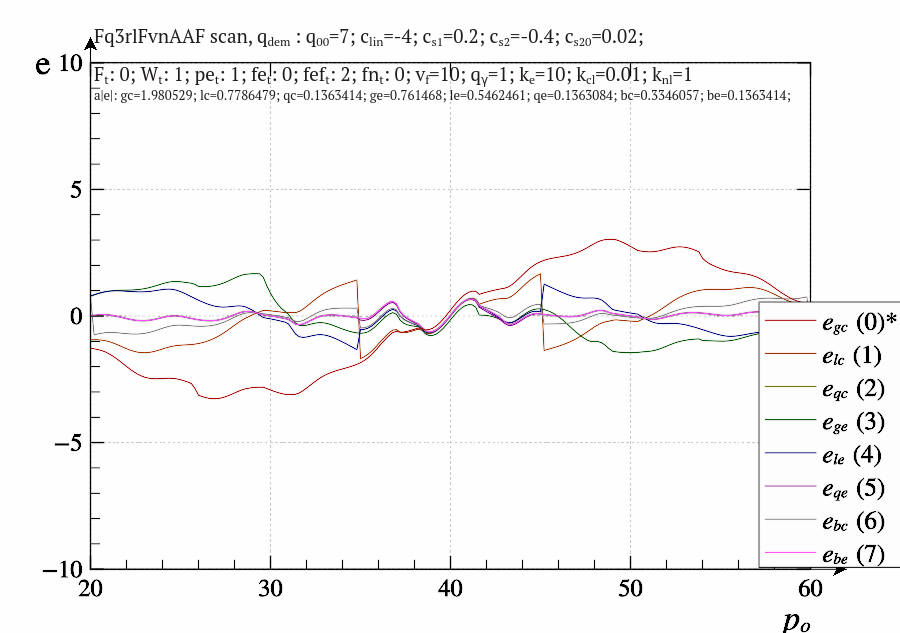
\includegraphics[width=0.7\textwidth]{p3/p/scan/qls-p_p_e_Fq3rlFvnAAF_scan.png}
  }
  \caption{Залежності $ e (p_o) $ для групи методів Fq3rlFvnAAF в квазістаціонарному випадку}
  \label{atu:f:Fq3rlFvnAAF_scan}
\end{figure}

На рис.~\ref{atu:f:ql3rlWvnAAW_scan} наведено залежності для групи методів ql3rlWvnAAW.
%
\begin{figure}[htb!]
  \centerline{
    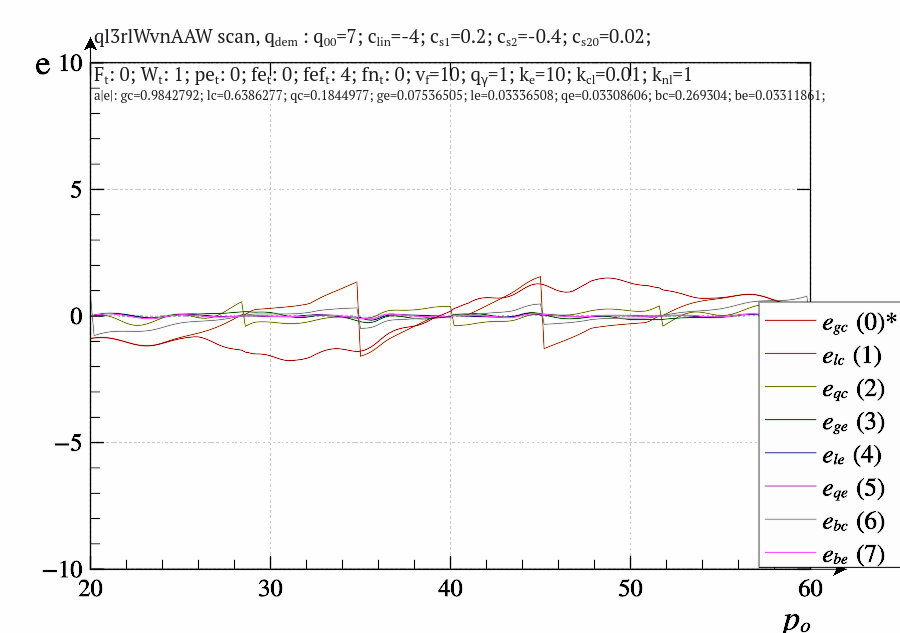
\includegraphics[width=0.7\textwidth]{p3/p/scan/qls-p_p_e_ql3rlWvnAAW_scan.png}
  }
  \caption{Залежності $ e (p_o) $ для групи методів ql3rlWvnAAW в квазістаціонарному випадку}
  \label{atu:f:ql3rlWvnAAW_scan}
\end{figure}

Істотною відмінністю методів ``ql3r\ldots'' є менший загальний рівень
помилок, а також відсутність похилого учаска залежності $ e (p_o) $ при
$ p_o \approx 40 $. В околиці цієї точки похідна приймає близьке до нуля значення, і
методи ``Fq3r\ldots'' не забезпечують належної чутливості в цій області, що
призводить до зростання помилки ідентифікації.
Таким чином, в квазістаціонарному випадку існує достатній набір працездатних
методів. При наявності можливості, слід використовувати методи, які
використовують величину критерію, на рівні координатора --- $ p_e $, і
наприклад, $ W $. Вибір інших елементів класифікації повинен проводиться
виходячи з інших умов, наприклад, вимог до динамічних характеристик системи
ідентифікації.

Для дослідження динамічних властивостей розглянутих методів ідентифікації без
прив'язки до конкретного об'єкта, будемо вважати, що для тестової задачі
характерний час стабілізації критерію значно менше характерних часів процесів
пошуку.
Таким чином, будемо розглядати тестове завдання~(\ref{atu:eq:q_dem}),
заданий повний набір коефіцієнтів, а динаміка параметра описується меандром~(\ref{atu:eq:po_t_sign}).
При цьому для аналізу буде використовуватися тільки один фронт~$p_o(t)$.

Для оцінки динамічних властивостей методів ідентифікації необхідна природна
одиниця часу, яка визначається самою системою ідентифікації. В якості такої
одиниці пропонується використовувати час, за яке агент перетинає всю свою
робочу смугу, за умови, що $ f_e $ зберігає максимальне можливе значення під
час руху, іншіми силами нехтуємо. Тоді цей час визначається наступним чином:
%
\begin{equation}
  t_{ua} = \frac{p_r - p_l}{ v_f k_e (p_r - p_l)} = \frac{1}{v_f k_e}.
  \label{atu:eq:t_ua}
\end{equation}
%
У розглянутих прикладах $t_{ua} = 0.01$.

Динаміка агентів і значень ідентифікованих параметрів для групи методів
``Fq3rlovnAAW'' і вищевказаних умовах приведена на рис.~\ref{atu:f:Fq3rlovnAAW_sign}.

\begin{figure}[htb!]
  \centerline{
    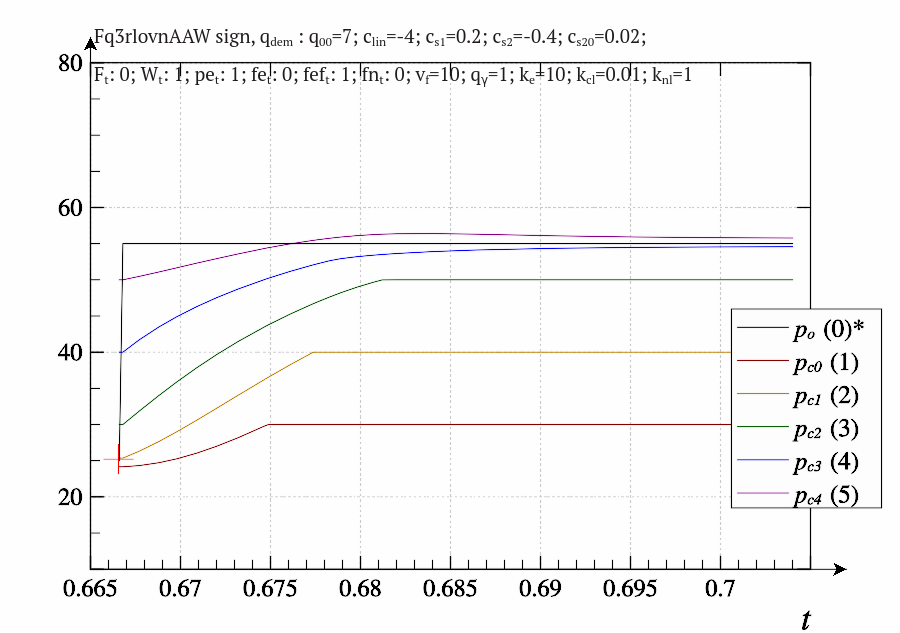
\includegraphics[width=0.45\textwidth]{p3/p/sign/qls-p_t_pi_m_Fq3rlovnAAW_sign.png}
    \hfill
    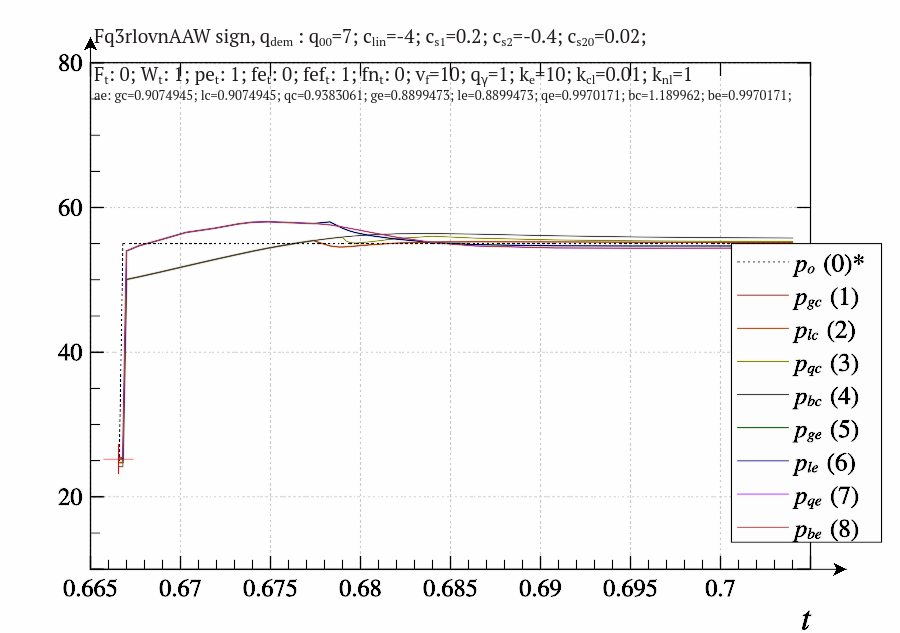
\includegraphics[width=0.45\textwidth]{p3/p/sign/qls-p_t_p_m_Fq3rlovnAAW_sign.png}
  }
  \caption{Динамика реакції агентів та $p_\mathrm{id}$ на стрибок параметру для групи методів ``Fq3rlovnAAW''}
  \label{atu:f:Fq3rlovnAAW_sign}
\end{figure}

Ця група методів характеризується одиничним множником у визначенні $ f_e $, що,
з одного боку, дає можливість агентам зміщуватися з максимальною швидкістю, з
іншого --- призводить до того, що ``далекі'' агенти зміщуються сильно,
займаючи місце поблизу кордону своєї робочої смуги. Як наслідок --- після
стрибка параметра поблизу положення, відповідного новому значенням, немає
досить близько розташованого агента, що збільшує час реакції системи.


Використання  групи методів ``ql3rlWvnAAW'',
приводить до більш сприятливої до ідентифікації динамічних систем ситуації
(рис.~\ref{atu:f:ql3rlWvnAAW_sign}).

\begin{figure}[htb!]
  \centerline{
    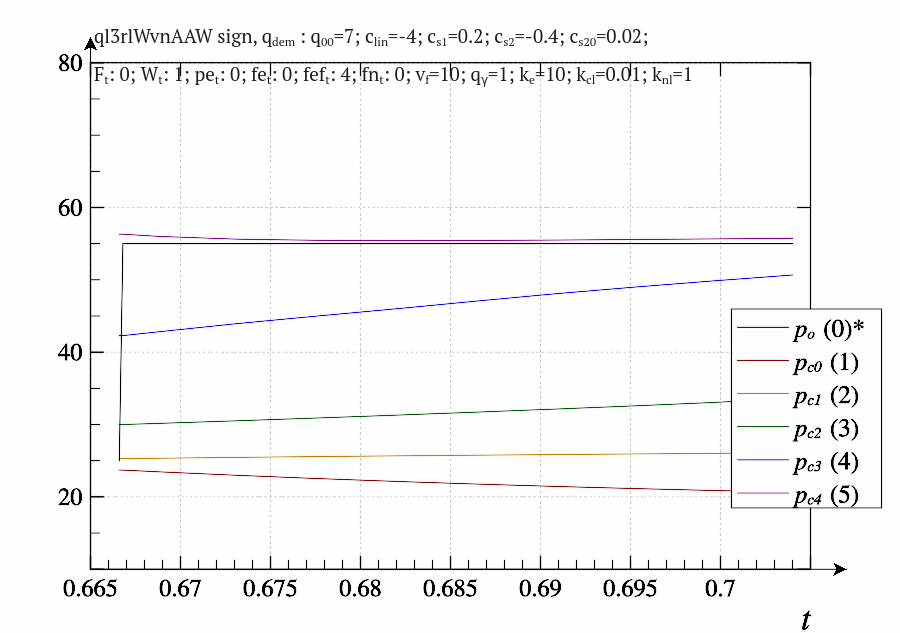
\includegraphics[width=0.45\textwidth]{p3/p/sign/qls-p_t_pi_m_ql3rlWvnAAW_sign.png}
    \hfill
    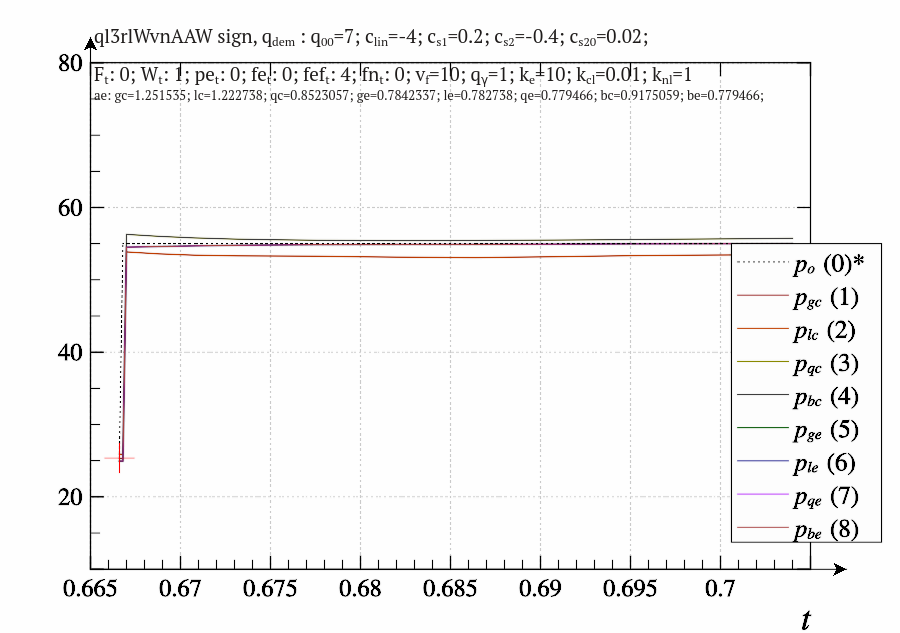
\includegraphics[width=0.45\textwidth]{p3/p/sign/qls-p_t_p_m_ql3rlWvnAAW_sign.png}
  }
  \caption{Динамика реакції агентів та $p_\mathrm{id}$ на стрибок параметру для групи методів ``ql3rlWvnAAW''}
  \label{atu:f:ql3rlWvnAAW_sign}
\end{figure}

Як вже було зазначено, використання у визначенні $ f_e $ значень $F$, $W$,
не дозволяє ``далеким'' агентам зміщуватися занадто сильно. Така відмінність
призводить до того що всі розглянуті методи дуже швидко (у порівнянні з $ t_{ua} $)
стабілізуються в околиці свого кінцевого значення. Відмінність
проявляється лише в тому, яке це значення. Методи, які використовують значення
$ p_c $ агента, характеризуються дещо більшими помилками помилками
ідентифікації. З іншого боку, методи, які використовують $ p_e $ агентів,
характеризуються практично однаковою низькою помилкою ідентифікації.

Для даної тестової задачі принципових відмінностей між групами методів
``ql3rlFvnAAW'', ``ql3rlSvnAAW'' і ``ql3rlWvnAAW'' не спостерігається. Для
реальних завдань ідентифікації відмінності можуть бути істотніше.





\medskip
\textbf{У третьому розділі}
розглядається розроблене програмне
забезпечення
для моделювання
поведінки  нелінійних,
у тому числі хаотичних динамічних систем.
Програма ``qontrol'' була створена для моделювання динаміки
нелінійних систем та проведення аналізу.

Мова програмування --- C++,
графічний інтерфейс реалізовано за допомогою
бібліотек Qt, gsl та mathGL.
Розроблено ієрархію класів для
моделювання різноманітних елементів,
у тому числі суттєво нелінійних.

Також було створено спеціалізоване
програмне забезпечення для мікроконтролерів,
щодо забазпечення взаємодії
з реальнии динаміними системами.




\textbf{У четвертому розділі}
розглянуте практичне застосування розроблених методів при моделюванні
процесів ідентифікації ряду систем хаотичної динаміки,
ак відомих, так і тих, які розглянуто вперше.

У якості першої ідентифікованої хаотичної системи розглянемо класичну систему
Лоренца, динаміка якої описується системою рівнянь:
%
\begin{equation}
\begin{cases}
  \dot{x} = \sigma (y-x ) , \\
  \dot{y} = x (r-z) - y , \\
  \dot{z} = x y - b z .
\end{cases}
\label{atu:eq:lor}
\end{equation}

Найціннішим з точки зору ідентифікації є параметр $ r $, що визначає як
енергетичний стан системи, так і вид динаміки системи. Це підтверджують і
фізичні обгрунтування. Для визначеності задамо інші параметри наступним
класичним чином: $ b = 2.6666667 $, $\sigma = 10 $, якщо не буде явно
зазначено протилежне.

При малих значеннях параметра $ r $ система демонструє затухаючі коливання.
Далі, в широкому діапазоні значення параметра $r$ система проявляє хаотичну
динаміку. Крім цього, спектр даної системи в хаотичному режимі досить широкий
(рис.~\ref{atu:f:lor_attractor_phase_chaos28}) і не має домінуючих
частот, що не характерно для багатьох систем динамічного хаосу.
При подальшому зростанні параметра $ r $ динаміка системи стає
складно-періодичної, з явно вираженим лінійчатим спектром.

\begin{figure}[ht!]
\begin{center}
  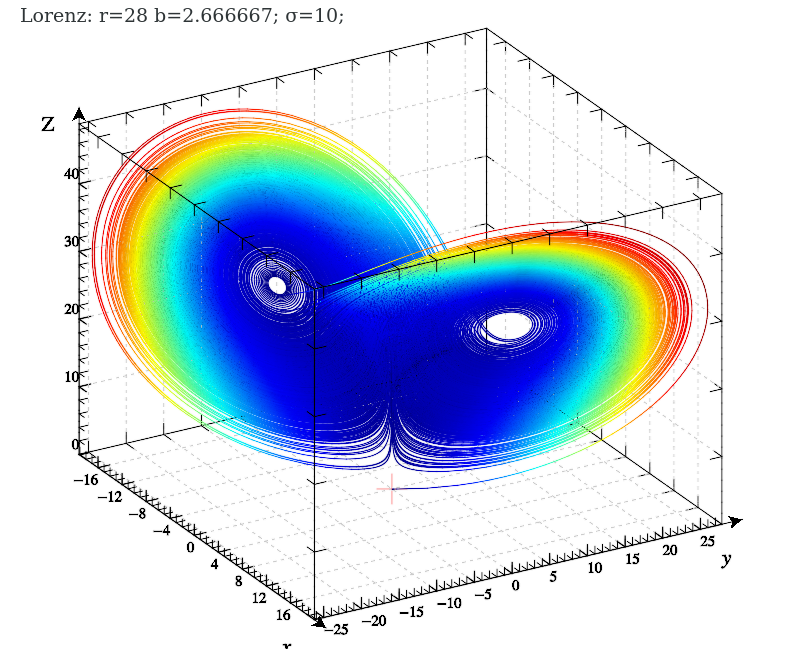
\includegraphics[width=0.45\textwidth]{p5/p/cha/lor/lor0-p_xyz_r=028.png}
  \hfill
  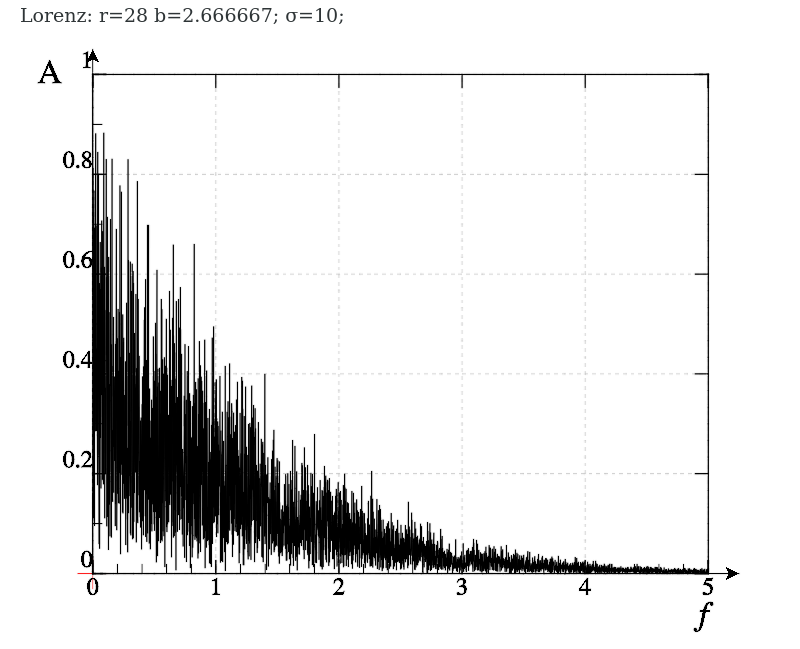
\includegraphics[width=0.45\textwidth]{p5/p/cha/lor/lor0_fft-p_f_r=028.png}
\end{center}
  \caption{Аттрактор і спектр системи Лоренца (\ref{atu:eq:lor}) в хаотичному режимі($r=28$)}
\label{atu:f:lor_attractor_phase_chaos28}
\end{figure}

Для синтезу критерію ідентифікації параметра $ r $ системи
(\ref{atu:eq:lor}), розглянемо набір фізичних систем, для моделювання яких застосовується
система Лоренца. Історично першою такою системою є завдання про теплової
конвекції рідини в плоскому шарі.
Змінні і параметри системи Лоренца визначаються наступним чином: $ x $ задає
швидкість обертання валів течії, $ y $, $ z $ --- відповідають розподілу
температури по горизонталі і вертикалі. $ \sigma $ --- число Прандтля
(відношення коефіцієнтів кінематичної в'язкості і температуропровідності).
Параметр $ b $ визначає відносини розмірів осередку. $ R $ --- (ідентифікований
параметр) --- наведене число Релея, що визначає енергетичні параметри
конвективного течії.
З трьох змінних стану найпростіше спостереження піддається змінна $ x $.
З іншого боку, так як параметр $ r $ визначає енергетичні співвідношення в
системі, то і критерій якості повинен являти собою квадратичну форму від $ x $,
причому усереднену на інтервалі часу, значно більшому, ніж характерний час
обороту рідинного вала.

Виходячи з вищевикладеного, в першу чергу слід перевірити придатність критерію
виду $ q_ {x ^ 2} $. Проте, перевіримо всі критерії даного виду, застосовні до
даної системи. На рис.~\ref{atu:f:lor_q} наведені досліджувані залежності
$q_{*}(r)$.

\begin{figure}[ht!]
  \centerline{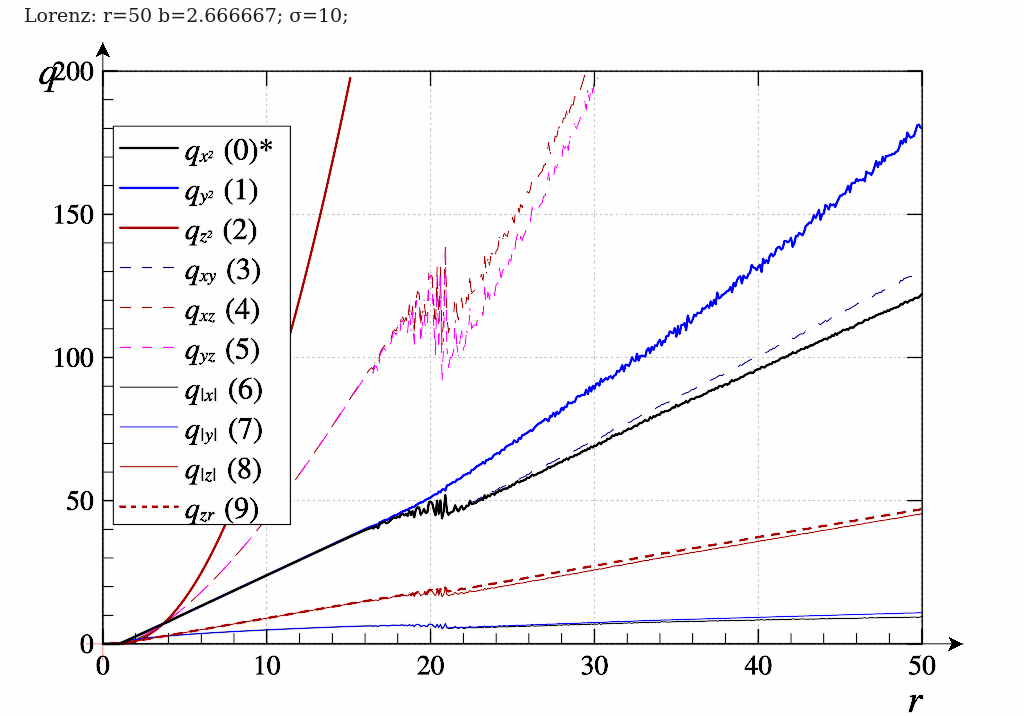
\includegraphics[width=0.5\textwidth]{p5/p/cha/lor/lor_q-p_q_r.png} }
  \caption{Розглянуті критерії для системи Лоренца}
  \label{atu:f:lor_q}
\end{figure}

Аналіз графіків дозволяє зробити висновок, що практично всі розглянуті види
критеріїв повинні дозволяти побудувати працездатну систему ідентифікації. При
цьому, велика частина графіків, в тому числі і з самого початку запропонований
$q_{x^2}$, втрачають монотонність при переході від режиму загасаючих
коливань до хаотичного.
Спектри сигналів $ x (t) $, $ y (t) $ і $ z (t) $ мають практично однакову
структуру. У подальших дослідженнях обмежимося критеріями
$q_{x^2}$ и
$q_{y^2}$.
Також отримано залежності $ \sigma_q(\tau_q) $ та  $ \sigma_q(a_q) $,
що доволяє корректно установити $a_q$.

Визначимо тестове завдання наступним чином:
\[
  p(t) \in [20, 60],
\]
%
\begin{equation}
  r_o(t) = p_o(t) = p_0 +  U_{p} \sign \sin( \omega_{p} t ),
  \label{atu:eq:lor_po_t_sign}
\end{equation}
%
%
\begin{equation}
  r_o(t) = p_o(t) = p_0 +  U_{p} \sin( \omega_{p} t ),
  \label{atu:eq:lor_po_t_sin}
\end{equation}
%
де:
$p_0 = 37$, $U_p=12$, $\omega_p=0.09$.

Рассморено застосування для ідентфікаціі методу з одним агентом, керуючим двома
моделями, і використовує два УГПК і інтегратором для визначення динаміки агента
(``Fl2nlosdlcA.$q_{x^2}$''). Встановлено, що він
працездатний, аде
не забезпечує потрібної швидкодії.
Для порівняння були обрані три групи мультімодельних метода ідентифікації:
ql3ruonAAF.$q_{x^2}$,
ql3ruonAAF.$q_{y^2}$ и
Fq3zlovnAAF.$q_{x^2}$.
На рис.~\ref{atu:f:lor_id_ql3ruonAAF.q_x2_sign} представлені результати
ідентифікації методом ql3ruonAAF. $q_{x^2} $, при цьому на лівому графіку
зображено динаміку переміщення кожної з рухливих моделей, а на правому -- 4
способи визначення $ p_\mathrm{id} (t) $.

\begin{figure}[ht!]
  \centerline{
    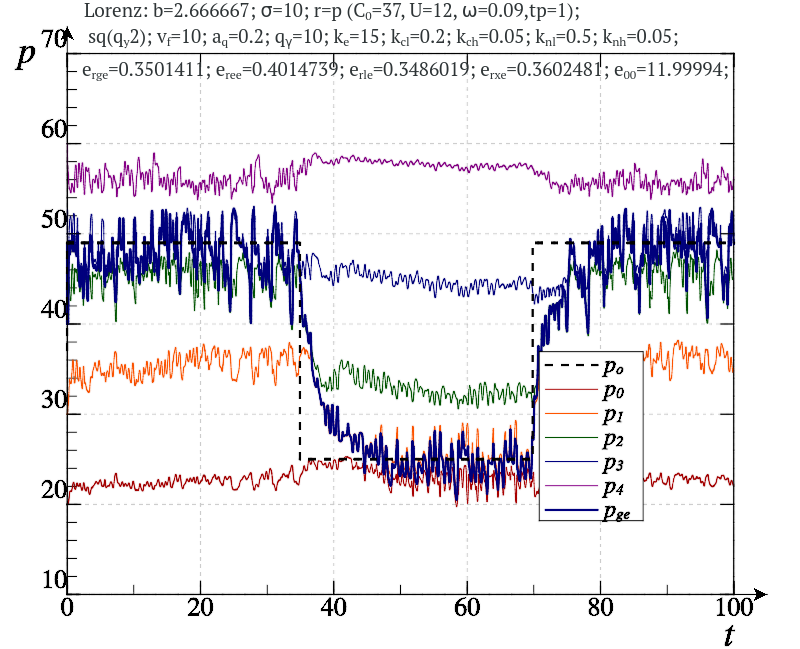
\includegraphics[width=0.45\textwidth]{p5/p/cha/lor/ql3ruonAAF/lor_ql3ruonAAF_qy2-p_t_pi_sign.png}
    \hfill
    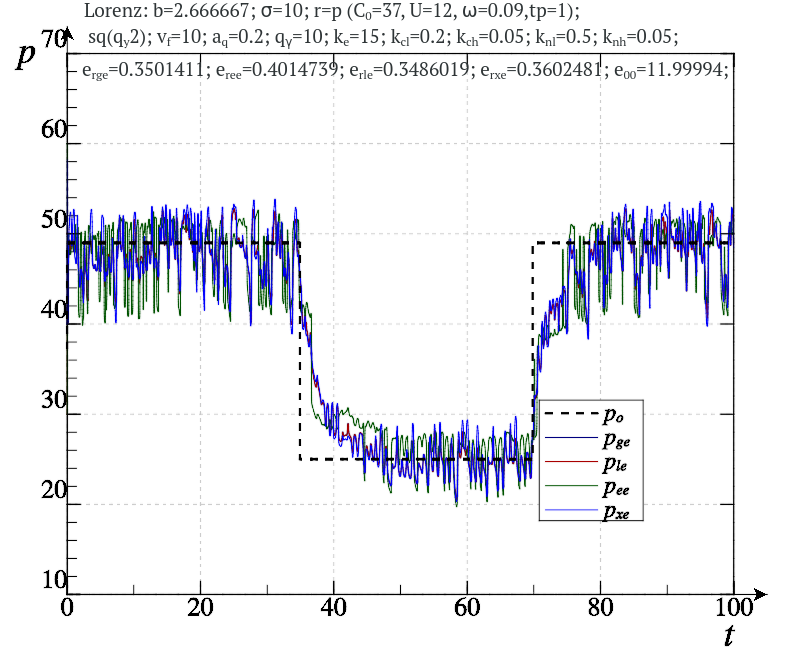
\includegraphics[width=0.45\textwidth]{p5/p/cha/lor/ql3ruonAAF/lor_ql3ruonAAF_qy2-p_t_pz_sign.png}
  }
  \caption{Процес ідентифікації параметра ``$r$'' системи Лоренца методом ql3ruonAAF.$q_{x^2}$ при умовах~(\ref{atu:eq:lor_po_t_sign})}
  \label{atu:f:lor_id_ql3ruonAAF.q_x2_sign}
\end{figure}

Найгірші результати демонструє $ p_{ge} $. Також, абсолютно очікувано, кращі
результати продемонстрував підхід $ p_{be}$. Також, при штучних обмеження
$v_f = 0 $ і $ q_\gamma = 0.1 $ були отримані величини, що характеризують
якість ідентифікації для нерухомих агентів:
$ \overline{e}_{bc} = 9.85 $ і
$ \overline{e}_{be} = 7.09 $, що свідчить про виправданість як переміщення
агентів, так і використанні величин $ p_e $ для визначення $ p_\mathrm{id} $.
Аналогічні результати, але з меншою помилкою ідентифікації були отримані за
умови плавної зміни значення параметра об'єкта~(\ref{atu:eq:lor_po_t_sin}).

Процес ідентифікації методом Fq3zlovnAAF за умовами~(\ref{atu:eq:lor_po_t_sign}) представлено
на рис.~\ref{atu:f:lor_id_Fq3zlovnAAF.q_x2_sign}. В першу чергу слід
відзначити велику рухливість агентів, аж до штучного обмеження рухливості
здебільшого моделей. З одного боку, це дещо зменшує швидкодію системи при
різких змінах параметра, з іншого --- забезпечує достатню зміщення ``далеких''
агентів, що, в якійсь мірі, компенсує можливі помилки в налаштуванні системи.

\begin{figure}[ht!]
  \centerline{
    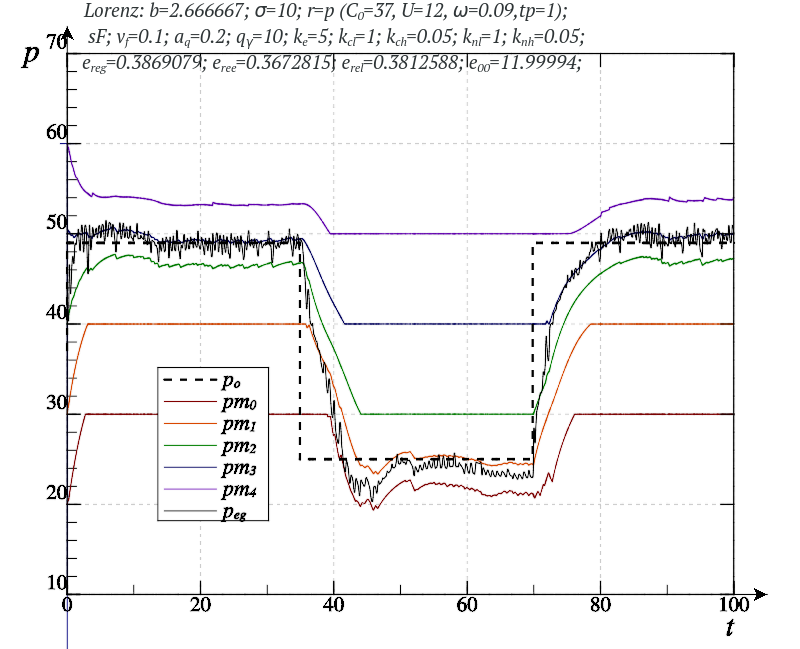
\includegraphics[width=0.45\textwidth]{p5/p/cha/lor/Fq3zlovnAAF/lor_Fq3zlovnAAF_qx2-pl_n_sign.png}
    \hfill
    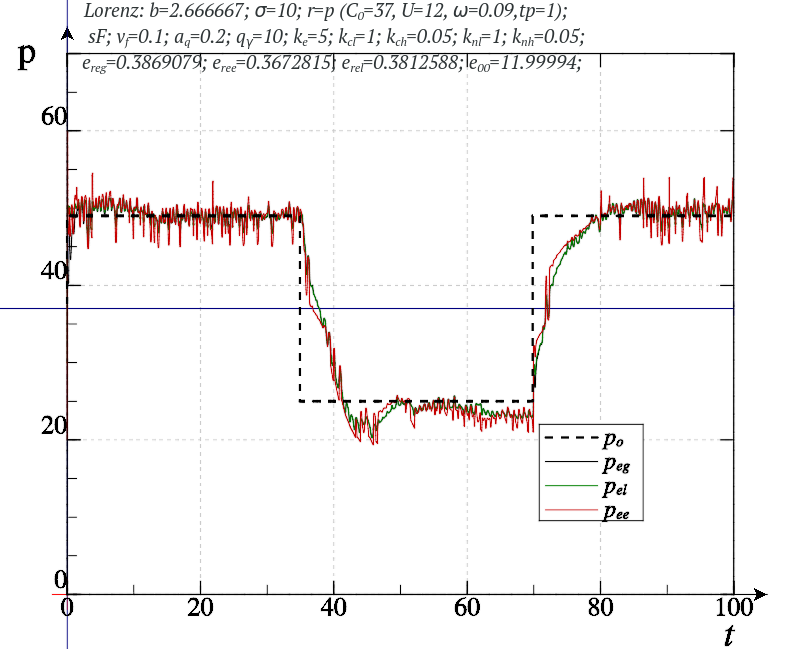
\includegraphics[width=0.45\textwidth]{p5/p/cha/lor/Fq3zlovnAAF/lor_Fq3zlovnAAF_qx2-p_p_sign.png}
  }
  \caption{Процес ідентифікації параметра ``$r$'' системи Лоренца методом Fq3zlovnAAF.$q_{x^2}$ при умовах~(\ref{atu:eq:lor_po_t_sign})}
  \label{atu:f:lor_id_Fq3zlovnAAF.q_x2_sign}
\end{figure}


Розглянуто вплив параметрів системи ідентифікації на процес ідентифікації. Для
цього будемо змінювався кожен з істотних параметрів і були побудовані
залежності $\overline {e}_{r*} $ для кожного з розглянутих методів.
Як приклад,
на рис.~\ref{atu:f:lor_a_q_ql3ruonAAF.q_x2} представлені залежності
усереднених помилок ідентифікації системи Лоренца від $ a_q $ при використанні
методу ql3ruonAAF.
Форма кривих з явним екстремумів обумовлена впливами протиборчих
факторів. При великих значеннях $ a_q $, занадто сильно вплив хаотичної
динаміки, що б можна було б проводити успішну ідентифікацію. З іншого боку, при
занадто малих значеннях $ a_q $, час оцінювання критерію настільки велике, що
система ідентифікації не встигає відслідковувати зміну параметра.

\begin{figure}[ht!]
  \centerline{
    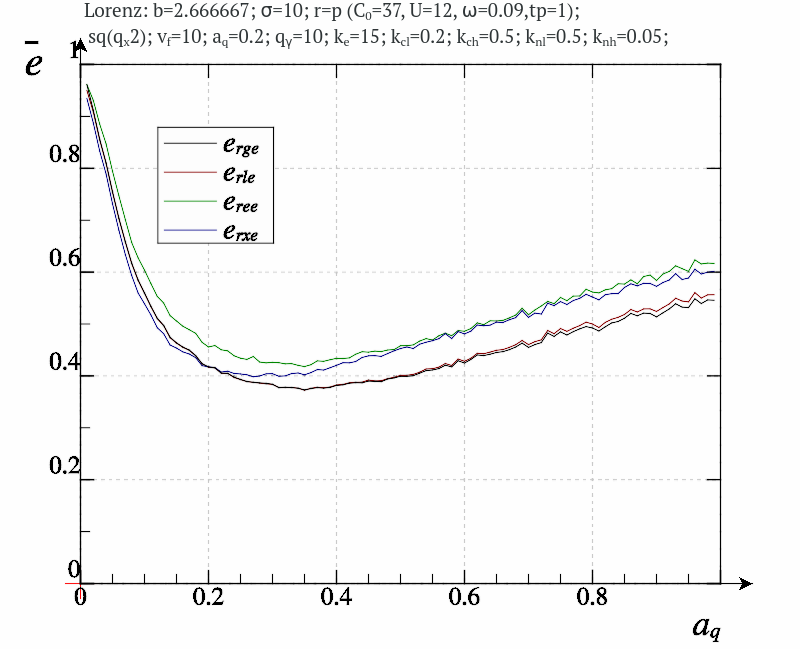
\includegraphics[width=0.45\textwidth]{p5/p/cha/lor/ql3ruonAAF/lor_ql3ruonAAF_qx2-p_a_q_e_sign.png}
    \hfill
    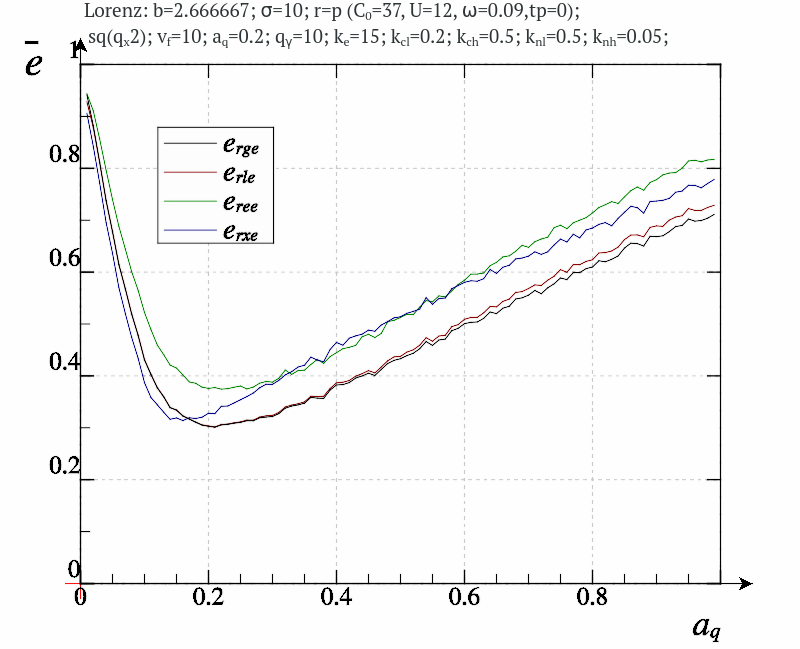
\includegraphics[width=0.45\textwidth]{p5/p/cha/lor/ql3ruonAAF/lor_ql3ruonAAF_qx2-p_a_q_e_sin.png}
  }
  \caption{Залежності $\overline{e}_{r*}(a_q)$ при ідентифікації системи Лоренца методом ql3ruonAAF.$q_{x^2}$
   при~(\ref{atu:eq:lor_po_t_sign}) и (\ref{atu:eq:lor_po_t_sin})}
  \label{atu:f:lor_a_q_ql3ruonAAF.q_x2}
\end{figure}

Також розглянуто вплив параметрів $q_\gamma$, $v_f$, $k_e$, $k_n$, $k_c$.
Визначено, що адаптивні властивості мульіагентних ансамблевих пошукових методів дозволяють
змінювати параметри системи ідентифікації в широких межах,
що спрощує настроювання ті забезпечую робастність метода.
Вид функыъ якості має вплив на результати, але не суттєвий.
Також встановлено, що як занадно мала, так і занадто велика кількість агентів
приводить до росту помилки ідентифікації.

Для оцінювання можливості одночасної ідентифікації декількох параметрів
розглянемо графіки залежностей критеріїв, але за умови зміни двох параметрів
попарно: ($ r $, $\sigma $) і ($ r $, $ b $).
На рис.~\ref{atu:f:lor_qz2_r_b}
приведена залежність
$q_{z^2}(r,b)$.
Близька до квадратичної залежність від параметра $ r $ не представляє особливих
проблем. Корисним є той факт, що для даного критерію залежність від параметра $b $
досить мала. Отже, при двупараметріческой ідентифікації даний критерій має
сенс використовувати для (оціночної) ідентифікації параметра $ r $, і
сукупність даного критерію разом з, наприклад, $ q_{x^2} $ дозволить
ідентифікувати обидва параметри без надмірної кількості моделей.

\begin{figure}[ht!]
  \centerline{  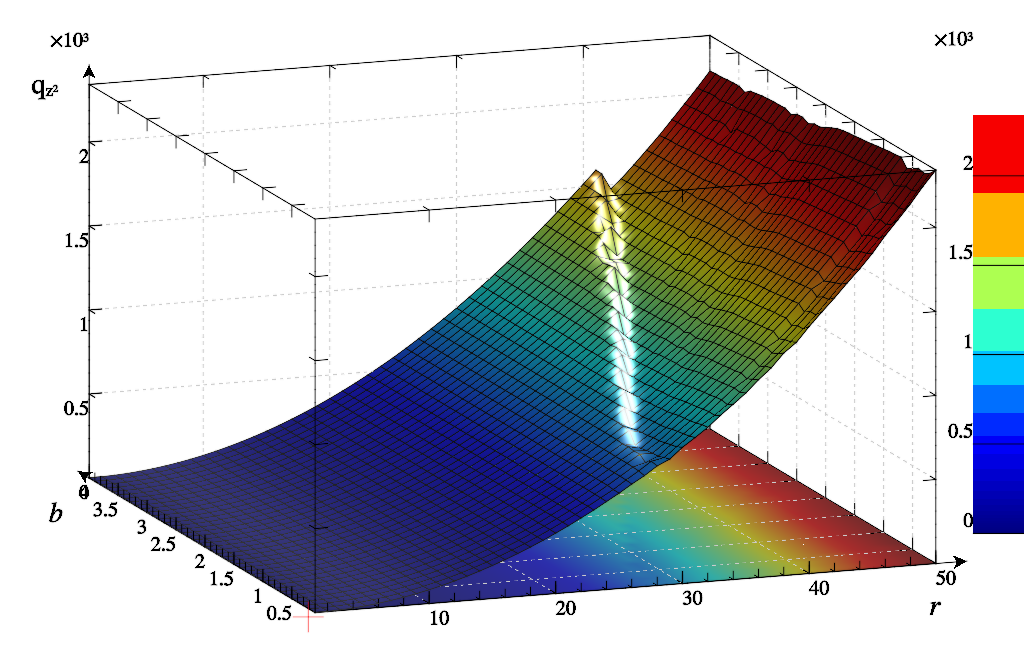
\includegraphics[width=0.50\textwidth]{p5/p/cha/lor/q2d/lor_qz2_r_b.png}  }
  \caption{Залежність $q_{z^2}(r,b)$ для системи Лоренца}
  \label{atu:f:lor_qz2_r_b}
\end{figure}


Таким чином,
для синтезу працездатної системи ідентифікації параметра ``$r$'' системи
Лоренца можуть застосовуватися практично все розглянуті критерії. При цьому,
більший діапазон застосовності --- у критерію  $q_{x^2}$.
Система мультиагентной ідентифікації може бути реалізована як з агентами, які
здійснюють пошук як з використанням критерію, так і з використанням функції
якості. При цьому, помилка ідентифікації визначається в основному не конкретним
методом, а динамічними властивостями самого ідентифікованого об'єкта і
використовуваним часом усереднення критерію.


Розглянемо систему, що позначається як ``Sprott A''~(\ref{atu:eq:spr_a_orig}). Відмінною
особливістю цієї системи є відсутність положень рівноваги, що унеможливлює
застосування багатьох відомих методів аналізу, заснованих на будь-якому
розкладі в околицях точок рівноваги.
%
\begin{equation}
  \begin{cases}
    \dot{x} =  y, \\
    \dot{y} = -x + yz, \\
    \dot{z} =  1 - y^2.
  \end{cases}
  \label{atu:eq:spr_a_orig}
\end{equation}

Додамо до системи параметр $c_{x_y}$:
%
\begin{equation}
  \begin{cases}
    \dot{x} =  c_{x_y} y, \\
    \dot{y} = -x + yz, \\
    \dot{z} =  1 - y^2.
  \end{cases}
  \label{atu:eq:spr_a}
\end{equation}

У такому вигляді система, при зміні $c_{x_y} $ в досить широкому діапазоні
може демонструвати як складно-періодичне, так і переважно, хаотичну поведінку
(рис.~\ref{atu:f:spr_a_p_0610}).

\begin{figure}[htb!]
\centerline{
  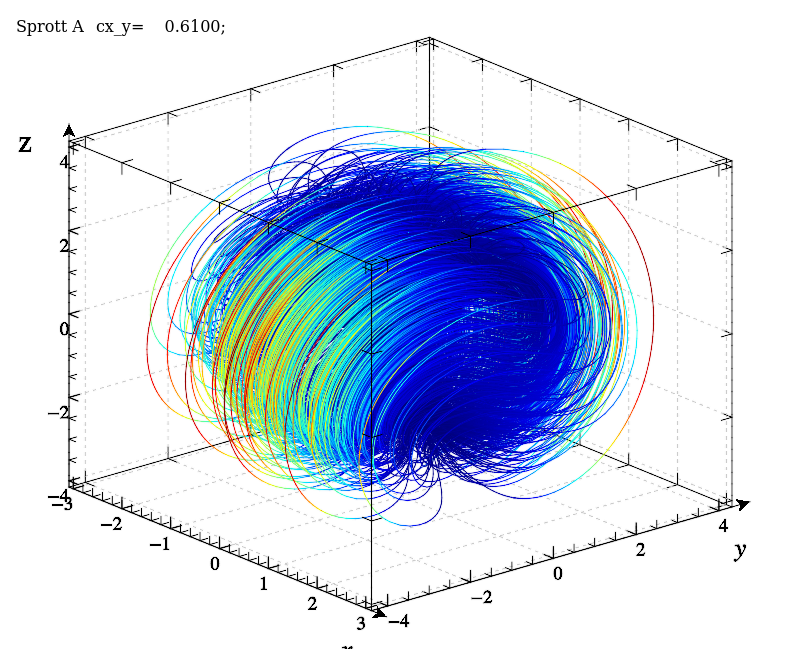
\includegraphics[width=0.45\textwidth]{p5/p/cha/spr_a/sprott_a-p_xyz_cx_y=0x610.png}
  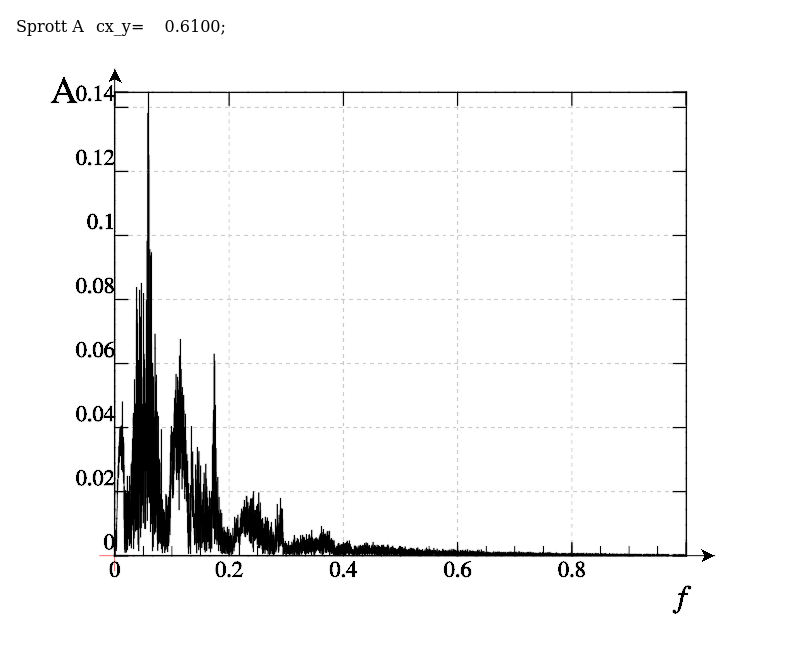
\includegraphics[width=0.45\textwidth]{p5/p/cha/spr_a/sprott_a_f-p_f_cx_y=0x610.png}
}
\caption{Атрактор та спектр системи (\ref{atu:eq:spr_a}) при $ c_{x_y} =0.610 $.
  Хаотичний режим
}
\label{atu:f:spr_a_p_0610}
\end{figure}


Розглянемо залежності $q_{*}(c_{x_y}) $ (рис.~\ref{atu:f:spr_a_q})
для системи (\ref{atu:eq:spr_a}). Аналіз цих залежностей дає практично
однозначну відповідь про можливий вид критерію --- $ q_{x^2} $.


\begin{figure}[htb!]
\centerline{
  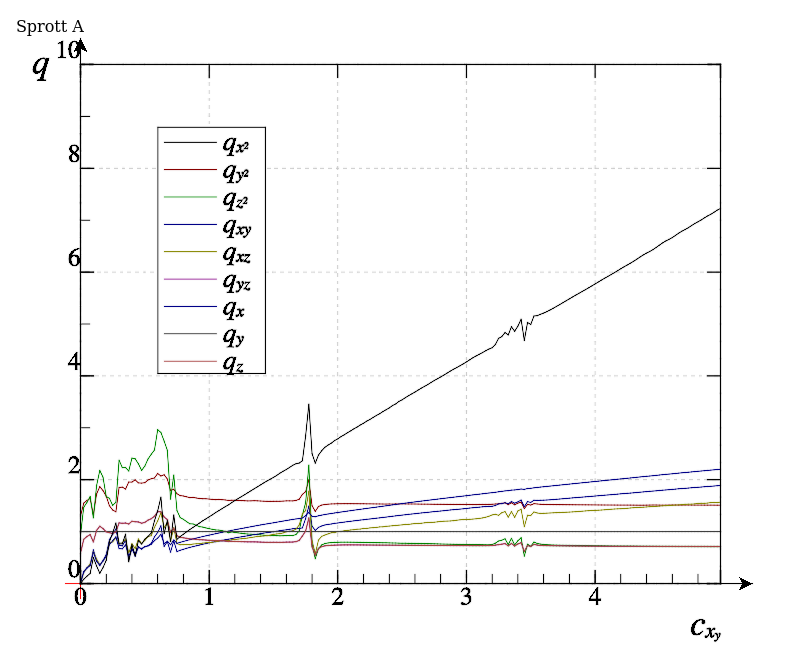
\includegraphics[width=0.50\textwidth]{p5/p/cha/spr_a/sprott_a_q-p_c_x_y.png}
}
\caption{Залежності $q_{*}(c_{x_y})$ для системы (\ref{atu:eq:spr_a}) }
\label{atu:f:spr_a_q}
\end{figure}

В околиці точки $ c_ {x_y} = 1.775 $ аттрактор також різко змінює свою
структуру. Так як це досить вузька околиця, то можна припустити, що
мультиагентна система ідентифікації не опиниться непрацездатною в цій області,
просто виросте помилка ідентифікації.

Визначимо тестове завдання наступним чином:
\[
  c_{x_y}(t) \equiv p_o(t) \in (0, 5],
\]
%
\begin{equation}
  p_o(t) = p_0 +  U_{p} \sign \sin( \omega_{p} t ),
  \label{atu:eq:spr_a_po_t_sign}
\end{equation}
%
%
\begin{equation}
  p_o(t) = p_0 +  U_{p} \sin( \omega_{p} t ),
  \label{atu:eq:spr_a_po_t_sin}
\end{equation}
%
де:
$p_0 = 2.8$, $U_p=1.9$, $\omega_p=0.04$.

На рис.~\ref{atu:f:spr_a_id_qAuv5.3r.q_x2_sign}
представлені результати моделювання процесу ідентифікації методом qAuv5.3r.
$q_{x^2} $. Залежність $ p_{xe} (t) $, в даному випадку демонструє високий
рівень коливань, і отже, гірші результати пошуку. При цьому, інші підходи до
визначення $ p_\mathrm{id} $ демонструють схожі між собою результати.

\begin{figure}[h!]
  \centerline{
    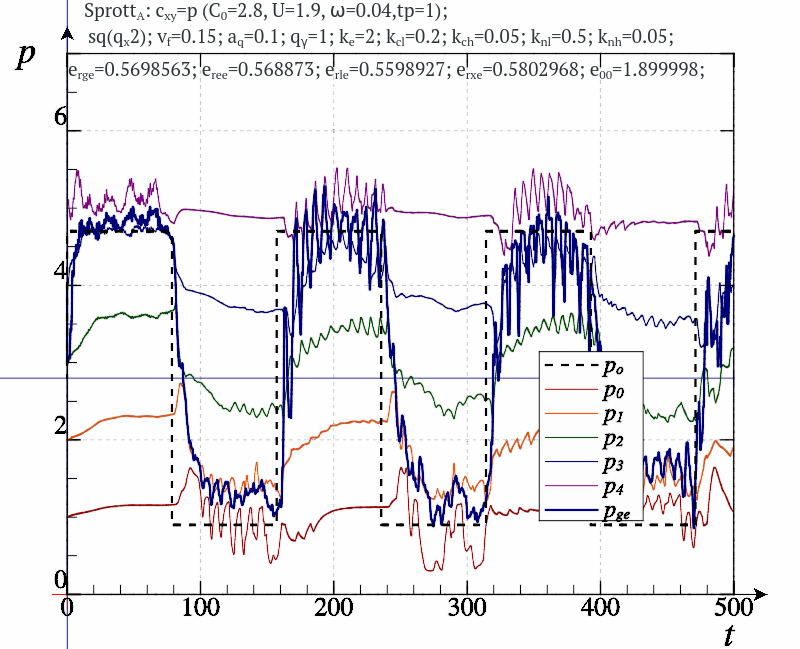
\includegraphics[width=0.45\textwidth]{p5/p/cha/spr_a/qAuv5.3r/sprott_a_qAuv5_3r_qx2-p_t_pi_sign.png}
    \hfill
    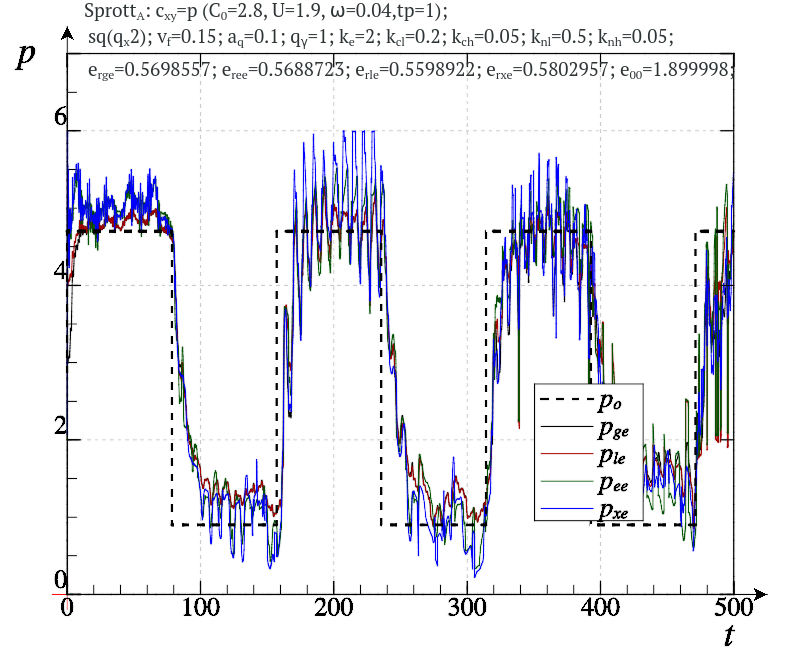
\includegraphics[width=0.45\textwidth]{p5/p/cha/spr_a/qAuv5.3r/sprott_a_qAuv5_3r_qx2-p_t_pz_sign.png}
  }
  \caption{Процес ідентифікації параметра ``$c_{x_y}$'' системы Sprott A методом qAuv5.3r.$q_{x^2}$ при умовах~(\ref{atu:eq:spr_a_po_t_sign})}
  \label{atu:f:spr_a_id_qAuv5.3r.q_x2_sign}
\end{figure}

На рис.~\ref{atu:f:spr_a_id_FAlv5.3r.q_x2_sign}
представлені результати ідентифікації методом
FAlv5.3r.$q_{x^2}$.


\begin{figure}[h!]
  \centerline{
    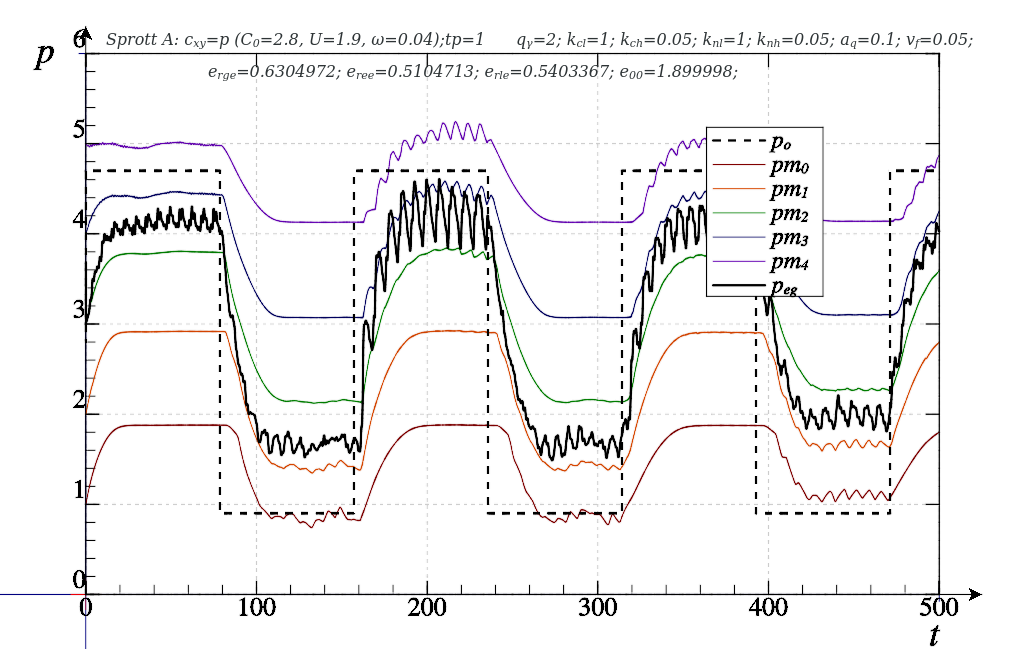
\includegraphics[width=0.49\textwidth]{p5/p/cha/spr_a/FAlv5.3A/sprott_a_FAlv5x3r-pl_n_sign.png}
    \hfill
    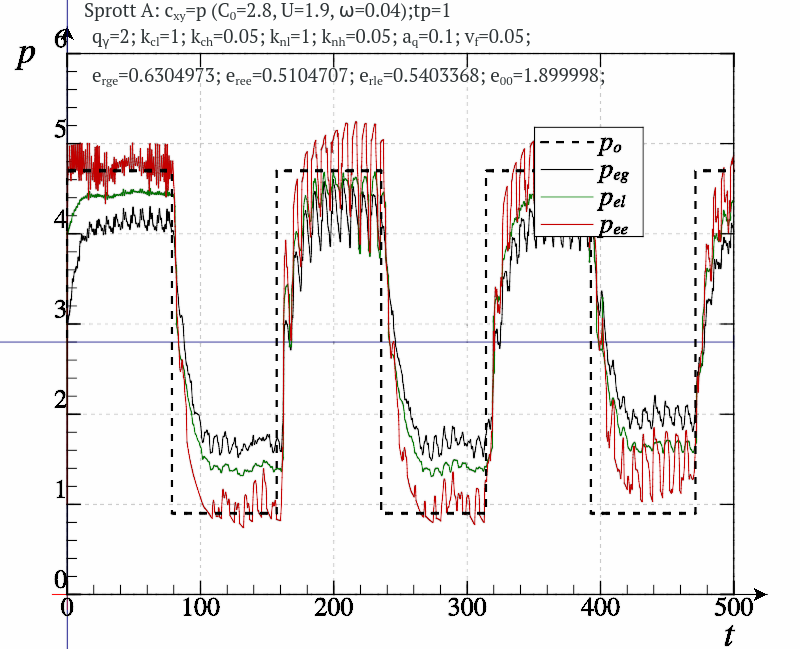
\includegraphics[width=0.49\textwidth]{p5/p/cha/spr_a/FAlv5.3A/sprott_a_FAlv5x3r-p_p_sign.png}
  }
  \caption{Процес ідентифікації параметра ``$c_{x_y}$'' системы Sprott A методом FAlv5.3r.$q_{x^2}$ при умовах~(\ref{atu:eq:spr_a_po_t_sign})}
  \label{atu:f:spr_a_id_FAlv5.3r.q_x2_sign}
\end{figure}

При наявності різниці у динамиці агентів, загальна помилка ідентификаціі
має той же порядок.

Також розглянуто вплив параметрів $a_q$, $q_\gamma$, $v_f$, $k_e$, $k_n$, $k_c$
на якість ідентифікації. Як і для системи Лоренца, методи
продемонстрували достатьню робастність, але для цієї системи
вплив динаміки агентів значно меньший.

Однією з відомих хаотичних систем, легко реалізованих як модельно
(\ref{atu:eq:chua}), так і схемотехнически, є нелінійна система Чуа:
%
\begin{equation}
\begin{cases}
  C_1 \dot{V_1}  = \frac{1}{R} ( V_2 - V_1 ) - g(V_1), \\
  C_2 \dot{V_2}  = \frac{1}{R} ( V_1 - V_2 ) + I_L, \\
  \dot{I_L}      = - \frac{1}{L} V_2 .
\end{cases}
\label{atu:eq:chua}
\end{equation}

Єдиним нелінійним елементом в цій системі є ``діод Чуа'' з характеристикою
$g(V)$~(\ref{atu:eq:diodchua}).
%
%
\begin{equation}
g(V) =
\begin{cases}
  m_1 V = ( m_0 + m_2 ) V , & |V| <   U_0, \\
  m_0 V ,                   & |V| \ge U_0.
\end{cases}
\label{atu:eq:diodchua}
\end{equation}

Введемо параметр \(m_2 = m_1 - m_0 \), який визначає в цілому нелінійність
системи. У даній роботі як ідентифікований параметра розглядається саме
параметр \(m_2 \).
Класично параметри системи Чуа задаються наступним чином:
$C_1 = 1/9$, $C_2 = 1$, $L= 1/7$, $R = 1/0.7$, $m_0=-0.5$, $ m_2 \in [ -0.15; -0.7 ] $.

Введемо позначення:
\[
  a_{11} = \frac{1}{R C_1}; \;
  a_{13} = \frac{1}{C_1}; \;
  a_{21} = \frac{1}{R C_2}; \;
  a_{23} = \frac{1}{C_2}; \;
  a_{31} = -\frac{1}{L}; \;
  a_g = - \frac{m_0}{C_1}; \;
  \mu = - \frac{m_2}{C_1}.
\]
%
%\noindent
Тоді
%
\begin{equation}
\begin{cases}
  \dot{V}_1  = -a_{11} V_1 + a_{11}  V_2  + g_1(V_1) , \\
  \dot{V}_2  = +a_{21} V_1 - a_{21}  V_2  + a_{23} I_L    , \\
  \dot{I}_L  =  a_{31} V_2.
\end{cases}
\label{atu:eq:chua2}
\end{equation}
%
%
\begin{equation}
g_1(V) =
\begin{cases}
  ( a_g + \mu ) V , & |V| <   U_0, \\
  a_g V           , & |V| \ge U_0.
\end{cases}
\label{atu:eq:diodchua2}
\end{equation}

\noindent
$ a_{11} = 6.5 $, $a_{21} = 0.7$, $ a_{23} = -7 $, $ a_g = 4.5 $,
$ \mu \in [ 1.29 ; 5.6 ] $.
Відповідно, в цих позначеннях ідентифікований параметр є~$\mu$.
Він задає динаміку системи (рис.~\ref{atu:eq:chua2}).

\begin{figure}[htb!]
\centerline{
  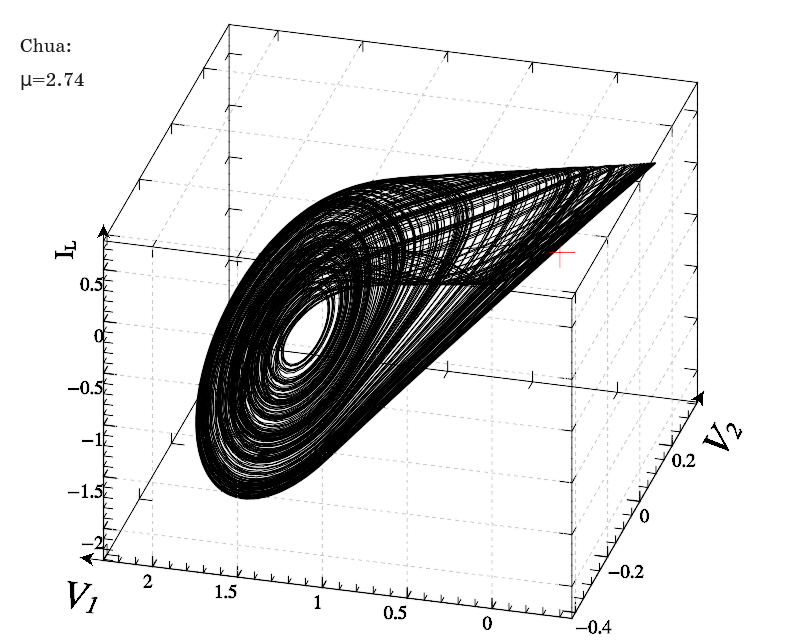
\includegraphics[width=0.45\textwidth]{p5/p/cha/chua/chua_1-p_xyz_mu=2x74.png}
  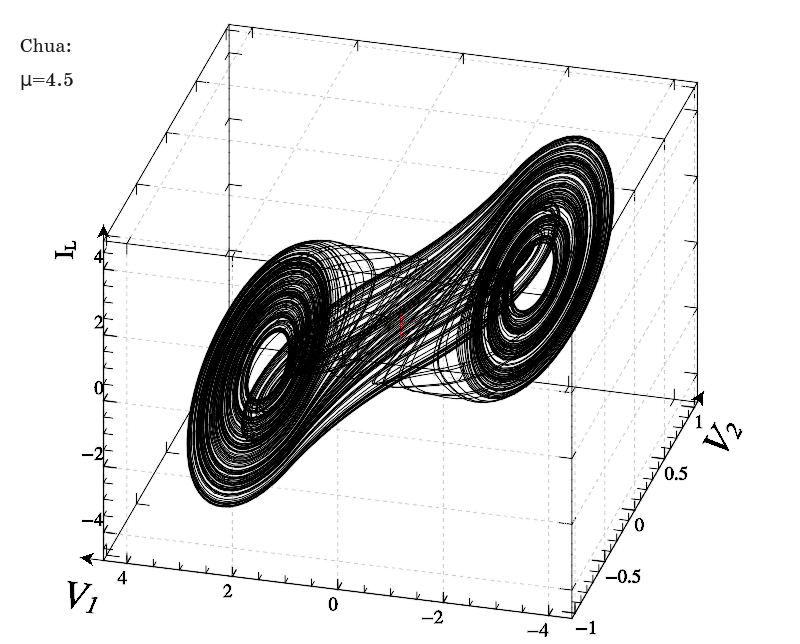
\includegraphics[width=0.45\textwidth]{p5/p/cha/chua/chua_1-p_xyz_mu=4x50.png}
}
\caption{Атрактор системи Чуа (\ref{atu:eq:chua2}) при різних значениях $\mu$}
\label{atu:f:chua_phase}
\end{figure}

Для визначення виду критерію розглянемо залежності $ q_{*}(\mu)$ отримані
шляхом моделювання для системи Чуа (рис.~\ref{atu:f:chua_q}):

\begin{figure}[htb!]
\centerline{
  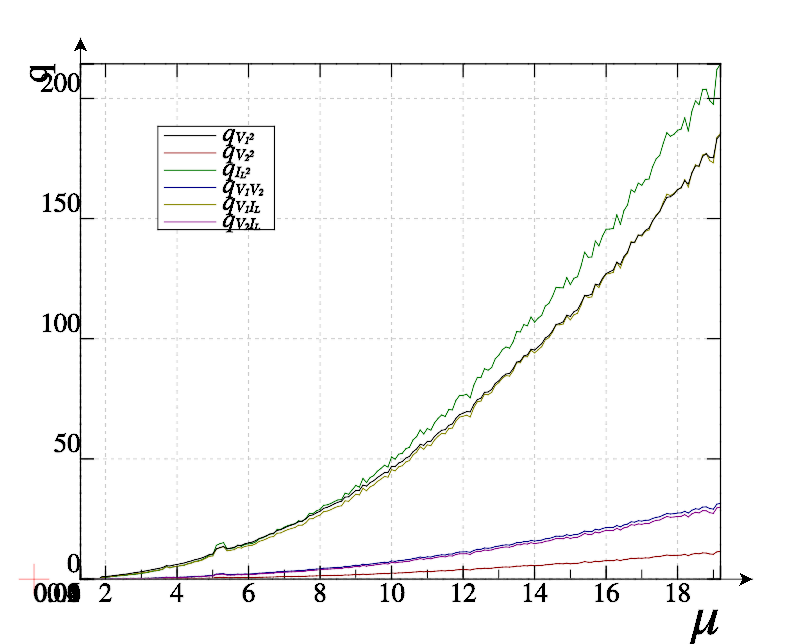
\includegraphics[width=0.45\textwidth]{p5/p/cha/chua/chua_q-p_mu2.png}
  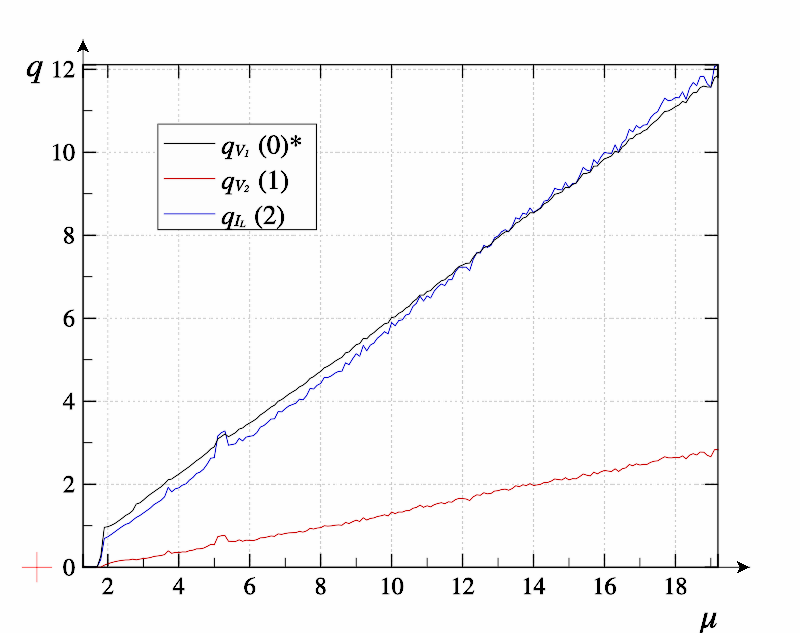
\includegraphics[width=0.45\textwidth]{p5/p/cha/chua/chua_q-p_mu1.png}
}
  \caption{Залежності $q_{*}(\mu) $ для системи Чуа (\ref{atu:eq:chua2})}
\label{atu:f:chua_q}
\end{figure}

З графіків очевидно, що величина $ q_{V_1} (\mu) $
є найкращим кандидатом в критерії, з огляду на близьку до лінійної залежності в робочому діапазоні.

Для ідентифікації використовувався метод ``Fq3rlovngcF''. Для
дослідження динамічних властивостей системи ідентифікації параметр $ \mu_o $
для об'єкта задавався двома способами:
%
\begin{equation}
 \mu_o(t) = p_0 + U_p \sign \sin( \omega_p t )
  \label{atu:eq:chua_mu_sign}
\end{equation}
%
\begin{equation}
 \mu_o(t) = p_0 + U_p \sin( \omega_p t ).
  \label{atu:eq:chua_mu_sin}
\end{equation}

Динаміка процесів ідентифікації для системи Чуа представлена на рис.~\ref{atu:f:chua_id}.

\begin{figure}[htb!]
\centerline{
  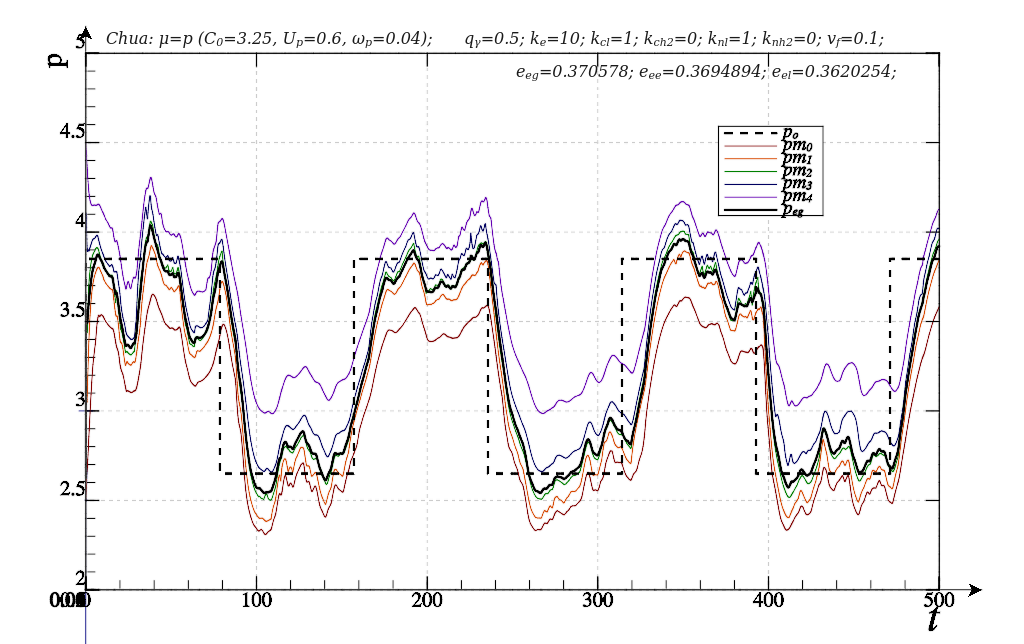
\includegraphics[width=0.45\textwidth]{p5/p/cha/chua/chua_m5p-pl_n_sign.png}
  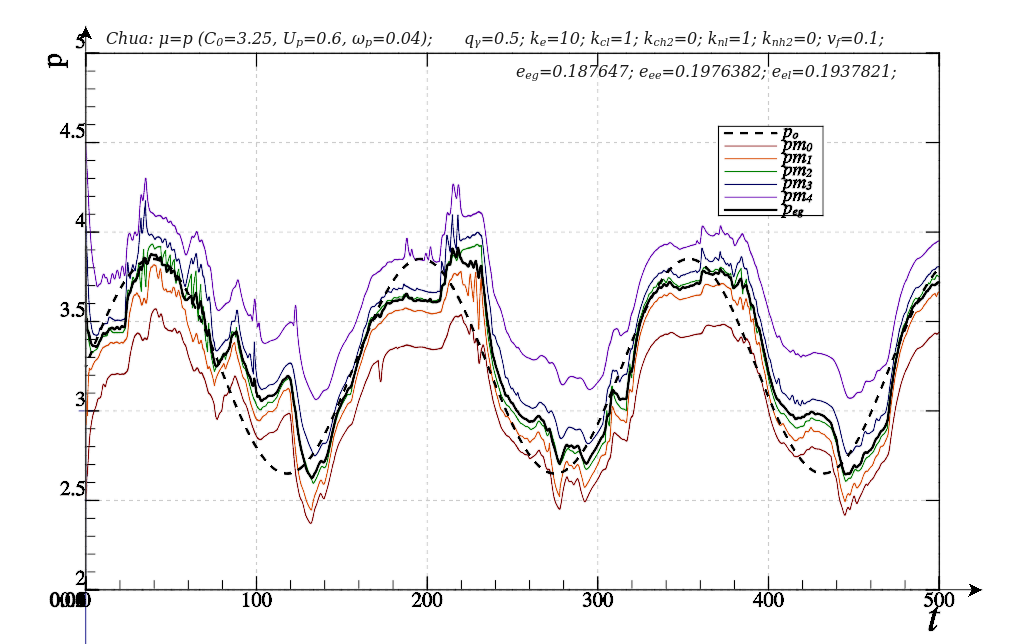
\includegraphics[width=0.45\textwidth]{p5/p/cha/chua/chua_m5p-pl_n_sin.png}
}
\caption{Процес ідентифікації параметра $\mu$ системы (\ref{atu:eq:chua2})
  при умовах (\ref{atu:eq:chua_mu_sign}) та (\ref{atu:eq:chua_mu_sin})
}
\label{atu:f:chua_id}
\end{figure}

Також розглянуто вплив параметрів $a_q$, $q_\gamma$, $v_f$, $k_e$, $k_n$, $k_c$
на якість ідентифікації. Методи
продемонстрували працездатність та робастність.


Існують динамічні системи, що не володіють хаотичним поведінкою, які, тим не
менш, проявляють подібні властивості з точки зору ідентифікації. А саме,
безпосереднє порівняння виходів системи і моделі не дозволяє зробити ніяких
висновків про співвідношення між параметрами моделі і об'єкта. Одним із
прикладів таких систем є динамічна система (\ref{atu:eq:dryfric_sys}), що
моделює поведінку тіла заданої маси по дією зовнішньої сили, що змушує і сили
сухого тертя
\cite{atu_asau11}:
%
\begin{equation}
  m \ddot{x} + f_{df}( x, \dot{x}, \ldots)  = u(t).
\label{atu:eq:dryfric_sys}
\end{equation}
%
%\noindent
де
$m$ -- маса тела,
$u(t)$ -- сила, що приводить до руху,
$ f_{df}( x, \dot{x}, \ldots)  $ -- сила сухого трения.

Важливою особливістю при моделюванні сили сухого тертя є той факт, що це силу
неможливо коректно висловити аналітично. Основним параметром, в найпростішому
випадку визначальним силу сухого тертя, є $f_{dm} $ --- максимальна значення її
модуля. Визначення цієї величини і будемо вважати метою завдання ідентифікації
системи з сухим тертям.

На рис.~\ref{atu:f:fric_outs}
представлено порівняльний приклад динаміки трьох моделей,
при однаковому вхідному сигналі і різних значеннях $ f_ {dm} $.

\begin{figure}[htb!]
  \centerline{
    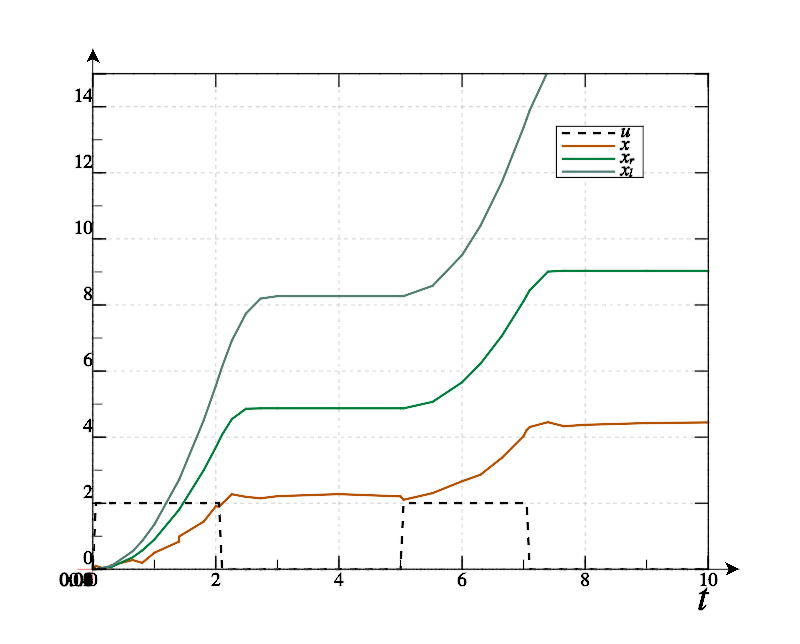
\includegraphics[width=0.4\textwidth]{p5/p/cha/fric/fric_outs.png}
  }
  \caption{Динаміка трьох моделей вида (\ref{atu:eq:dryfric_sys})}
  \label{atu:f:fric_outs}
\end{figure}

Для забезпечення можливості застосування методів ідентифікації, необхідно
існування критерію $ q (x (t)) $, що задовольняє наступним вимогам: чутливість
до динаміки моделі і об'єкта; властивість астатизма, достатня стійкість до
шумів вимірювання; фізична реалізація.

У даній роботі зробимо припущення, що рівень шумів дозволяє створити фільтр, що
дозволяє відсівати шуми за (як максимум) характерний час реакції системи. Після
фільтра діє реальне дифференцирующее ланка. Відповідний вид критерію позначимо як
$ q_{dx} $ (рис.~\ref{atu:f:fric_q}).

\begin{figure}[htb!]
\centerline{
  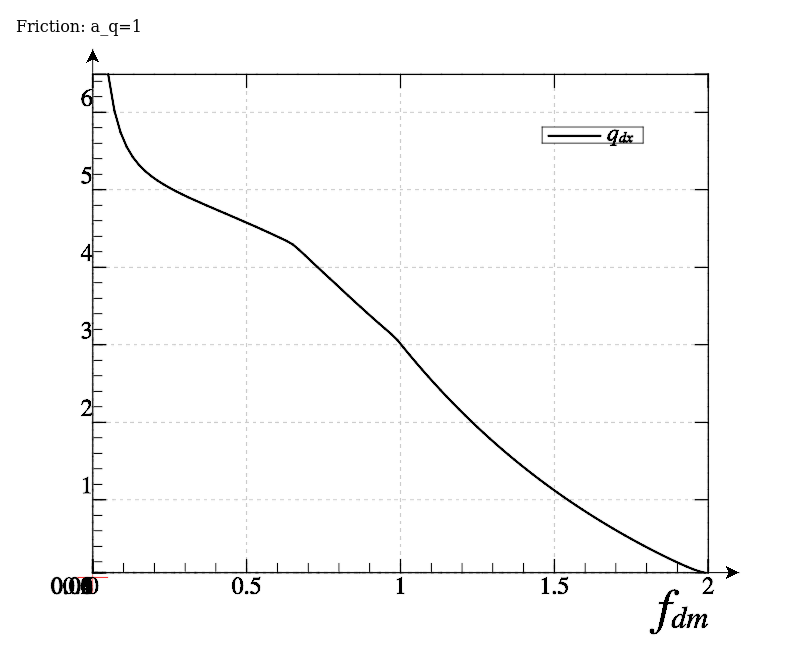
\includegraphics[width=0.40\textwidth]{p5/p/cha/fric/fric_p-p_f_dm_q.png}
}
  \caption{Залежність $q_{dx}(f_{dm})$ для системи (\ref{atu:eq:dryfric_sys}) }
\label{atu:f:fric_q}
\end{figure}


Динаміка процесів ідентифікації для системи (\ref{atu:eq:dryfric_sys})
представлена на рис.~\ref{atu:f:fric_id}. Слід зазначити
сильний вплив вхідного сигналу, В силу того, що коли системи нерухомі на одному
з ``плато'', то немає можливості розрізнити їх параметри, який б критерій при
цьому не використовувався.

\begin{figure}[htb!]
\centerline{
  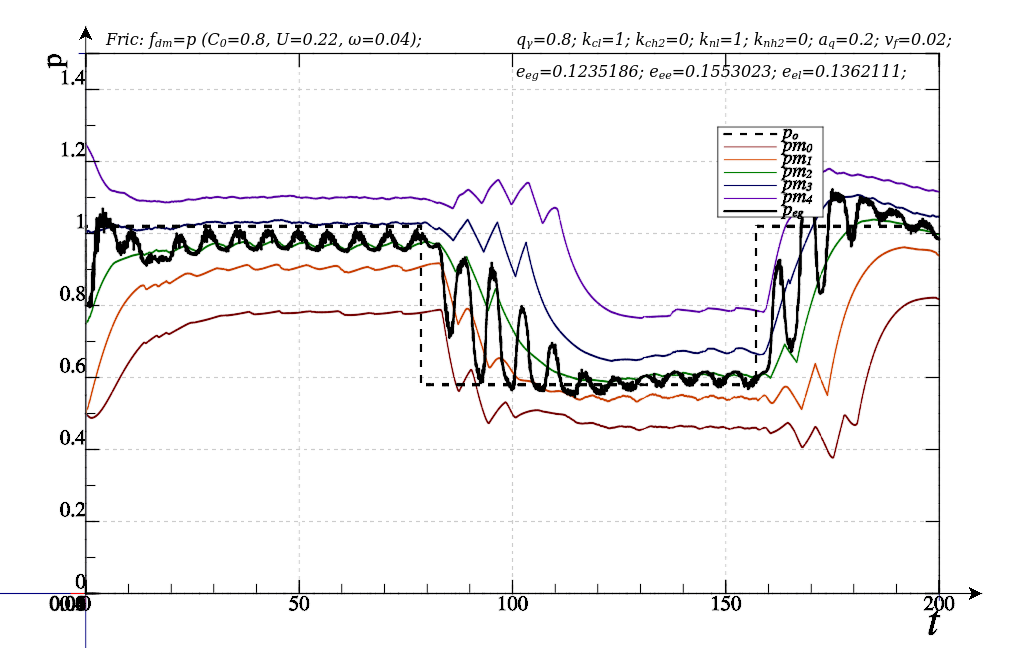
\includegraphics[width=0.45\textwidth]{p5/p/cha/fric/fric_m5p-pl_n_sign.png}
  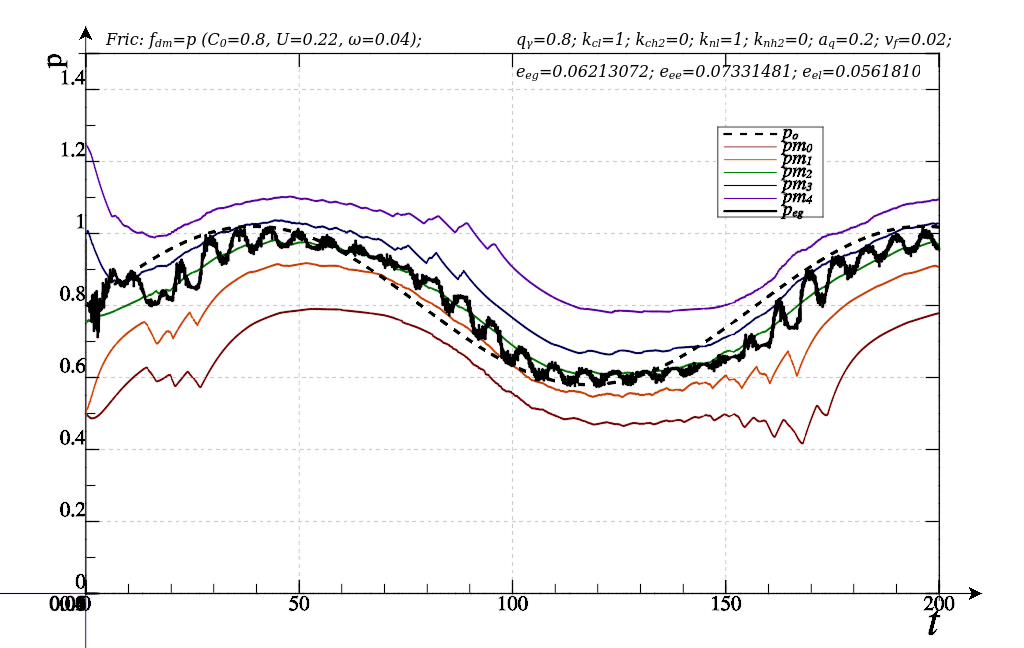
\includegraphics[width=0.45\textwidth]{p5/p/cha/fric/fric_m5p-pl_n_sin.png}
}
\caption{
  Процес ідентифікації параметра $ f_{dm} $ системи (\ref{atu:eq:dryfric_sys}) при різних видах нестаціонарності цього параметра
}
\label{atu:f:fric_id}
\end{figure}

Для даної системи енергетичні критерії, аналогічні застосованим в попередніх
випадках, виявилися незастосовні. Критерій, хоч і заснований на вимірюванні
похідною (після фільтрації), виявився працездатним. В першу чергу це пов'язано
з тим, що в основі були покладені фізичні принципи.





У підрозділі 4.3 досліджуються процеси ідентифікації системи Дуффінга.

У підрозділі 4.5 досліджуються процеси ідентифікації системи Ван-дер-Поля.

У підрозділі 4.6 досліджуються процеси ідентифікації системи Колпітца у традиційному вигляді.

У підрозділі 4.7 досліджуються процеси ідентифікації системи вібраційної системи
із зоною нечутливості у силі, що повертає.

У підрозділі 4.8 досліджуються процеси ідентифікації системи  вібраційної системи
із гістерезисом у силі, що повертає, у хаотичному режимі.

\textbf{У п'ятому розділі}
розглянуте практичне застосування
нових методів ідентифікації для генератора Колпітца
з використанням реального фізичного об'єкту.
Впроваджену нову математичну модель,
яка враховує більше нелінійних властивостей
BJT транзистора, та різних режимів роботи.

Створено мікроконтролерну систему, яка
дозволила отримати дані з реального
генератора, та за допомогою програмного комплексу,
який описано у розділі 3, перевірити адекватність як
нової моделі генератора, що було використано,
так і працездатність створеної для неї системи ідентифікації.



\textbf{У шостому розділі}
запропоновано модель
системи зв'язаних релаксаційних генераторів,
які проявляють хаотичну динаміку при певних умовах.
Досліджуються  властивості цієї системи.

Створено фізичний об'єкт,
який реалізовує запропановану динаміку,
а також
створено мікроконтролерну систему, яка
дозволила перевірити адекватність математичної моделі.
Також було проведено властивостей системи ідентифікації стосовно цієї системи.

\xsect{ВИСНОВКИ}

Основні результати дисертаційної роботи полягають у наступному:

\begin{itemize}

  \item
  створено нові критерії ідентифікації, які, на відміну від тих, що
  існують, придатні для аналізу стану та динаміки
  хаотичних систем, що створить фізично зумовлене обґрунтування працездатності систем
  ідентифікації;

  \item
  створено новий клас систем ідентификації у межах
    адаптивно-пошуковой парадигми,
    які за рахунок використання колективної динаміки
    ансамблю пошукових агентів забезпечують
    кращу якість ідентифицації;

  \item
  створено програмне забезпечення, придатне для моделювання як систем
  хаотичної динаміки, так і систем мультиагентної ідентифікації;

  \item
  проведено комп'ютерне моделювання процесів ідентифікації систем
  хаотичної динаміки, підтверджено їх працездатність.


\end{itemize}


\xsect{СПИСОК ОПУБЛІКОВАНИХ ПРАЦЬ ЗА ТЕМОЮ ДИСЕРТАЦІЇ}

\nocite{*}

\printbibliography[heading=none]




\xsect{АННОТАЦИЯ}

\textbf{\dissauthorRu}
\textbf{\booknameRu}
\textbf{--- На правах рукописи.}

Диссертация на соискание ученой степени
доктора
\dissScopeRu\ {}
по специальности
\dissSpecId\ --- <<\dissSpecRu>>.
\institutionRu, \belongRu, \cityRu, \bookyear.


Ключевые слова:
адаптивно-поисковая идентификация, нелинейные динамические системы,
информационные оценки, математическая модель.


\xsect{АНОТАЦІЯ}

\textbf{\dissauthorUa}
\textbf{\booknameUa}
\textbf{--- На правах рукопису.}

Дисертація на здобуття наукового ступеня
доктора
\dissScopeUa\ {}
за спеціальністю
\dissSpecId\ --- <<\dissSpecUa>>.
\institutionUa, \belongUa, \cityUa, \bookyear.


Ключові слова: адаптивно-пошукова ідентифікація, нелінійні динамічні
системи, інформаційні оцінки, математична модель.



\xsect{ABSTRACT}

\textbf{\dissauthorEn}
\textbf{\booknameEn}.
\textbf{--- As Manuscript.}

Thesis for the degree of Doctor of Technical Science in Specialization
\dissSpecId\ --- <<\dissSpecEn>>.
\institutionEn, \belongEn, \cityEn, \bookyear.

The dissertation is devoted to

Keywords: adaptive-search identification, nonlinear dynamic systems,
information estimations, mathematical model.

\clearpage

{~}
\vfill

\begin{center}


Підписано до друку xx.xx.\bookyear~р.

Формат $60 \times 84/16$  Папір друкарський. Ум. др.арк.~2

Друк різограф. Замовлення \No 02/17. Наклад --- 100 прим.

% ДНВП <<Системні технології>>

49006, Дніпро, пр.~Гагаріна,4

st@nmetau.edu.ua

\end{center}

\vfill


\end{document}

